\documentclass[UTF8,a4paper,zihao=5,fontset=none]{ctexart}
\usepackage[left=22mm,right=22mm,top=21mm,bottom=21mm,headheight=14pt,headsep=6mm]{geometry}
\usepackage{fontspec,amsmath,amssymb,bm,graphicx,booktabs,longtable,array,calc,multirow}
\usepackage[font=small,labelfont=bf,labelsep=space,justification=justified,singlelinecheck=false]{caption}
\usepackage{fancyhdr,enumitem,placeins,needspace,xurl,hyperref}
\hypersetup{hidelinks,pdftitle={基于候选交互与条件价值学习的多无人艇协同目标防御方法}}
\setmainfont{Liberation Serif}
\setCJKmainfont{Noto Serif CJK SC}
\setCJKsansfont{Noto Sans CJK SC}
\setCJKmonofont{Noto Sans Mono CJK SC}
\setlength{\parindent}{2em}
\setlength{\parskip}{2.5pt}
\linespread{1.17}
\setlength{\abovedisplayskip}{6.5pt}
\setlength{\belowdisplayskip}{6.5pt}
\setlength{\textfloatsep}{13pt}
\setlength{\intextsep}{12pt}
\setlength{\floatsep}{10pt}
\setlength{\LTpre}{4pt}
\setlength{\LTpost}{9pt}
\renewcommand{\arraystretch}{1.18}
\ctexset{section={format=\sffamily\bfseries\large,beforeskip=13pt,afterskip=6pt},subsection={format=\sffamily\bfseries\normalsize,beforeskip=10pt,afterskip=5pt},subsubsection={format=\sffamily\bfseries\normalsize,beforeskip=8pt,afterskip=4pt}}
\pagestyle{fancy}\fancyhf{}
\fancyhead[L]{\small 多无人艇候选交互与条件价值学习}
\fancyhead[R]{\small CIV-RL}
\fancyfoot[C]{\small\thepage}
\renewcommand{\headrulewidth}{0.35pt}
\setcounter{secnumdepth}{-2}
\setcounter{topnumber}{3}\setcounter{bottomnumber}{2}\setcounter{totalnumber}{5}
\renewcommand{\topfraction}{.92}\renewcommand{\bottomfraction}{.85}\renewcommand{\textfraction}{.08}\renewcommand{\floatpagefraction}{.75}
\emergencystretch=2em
\clubpenalty=10000\widowpenalty=10000
\providecommand{\tightlist}{\setlength{\itemsep}{0pt}\setlength{\parskip}{0pt}}
\begin{document}
\begin{center}\sffamily\bfseries\fontsize{18}{25}\selectfont
基于候选交互与条件价值学习的\\多无人艇协同目标防御方法
\end{center}\vspace{3pt}
\section*{摘要}

针对高机动攻击艇条件下多无人艇学习控制与规则控制的协同融合问题，提出候选交互与条件价值驱动的协同残差强化学习方法CIV-RL。以各艇左右推进器的融合系数为联合决策变量，根据候选控制的反馈预测轨迹构建艇对交互代价，联合确定艇队融合配置。利用相同初始状态和共同随机条件下的配对闭环结果，分别学习参考策略失败时的候选成功概率与参考策略成功时的候选失败概率，将两类成败转化组合为终局净收益，并据此选择完整融合方案。六艇数值试验中，所提方法在200个独立任务上取得90.0\%的防御成功率，较自适应残差基线提高25.5个百分点。共享候选集合与预测信息时，联合选择较独立选择提高8.5个百分点，艇间碰撞率由5.0\%降至2.5\%。在完整方法与CI参考策略共同捕获的176个任务中，平均捕获时间缩短0.83
s。12组Gazebo
VRX配对场景均完成捕获，冻结策略在5艇、7艇和8艇条件下分别完成23/24、22/24和19/24次防御。

\textbf{关键词}　多无人艇　协同目标防御　联合融合控制　候选运动交互　条件价值学习

\section*{1 引言}

多无人艇协同目标防御通过协调多个水面平台的机动，阻止入侵目标进入受保护水域，是海上设施防护和自主水面系统协作的重要研究问题{[}1,2,3{]}。攻击艇具有更高的加速、航速和转向能力时，防御艇需要在有限机动能力下保持对目标的接近，并兼顾拦截位置与艇间分离。当多艘防御艇同时接近相同拦截区域时，各艇局部有利的推进与转向选择可能形成近距交会，改变后续的捕获机会。单艇控制效果随其他防御艇的同时响应而变化，协同防御因而需要在完整艇队配置上协调局部控制选择。

围绕区域保护与协同追捕，已有研究从几何规划、追逃博弈和非线性控制等方面建立了拦截方法。区域防守策略依据攻击者的可达关系与目标边界确定防御机动，协同追捕方法将目标判断、任务规划和局部控制组织为连续的决策过程{[}2,3{]}。追逃博弈利用包围函数与双方运动能力刻画可捕获条件{[}4,5{]}，船舶神经控制进一步将非线性动力学引入对抗策略求解{[}6{]}。这类方法直接处理运动能力与拦截几何之间的关系。群体规则通过分离、对齐和聚合等局部作用生成协调运动{[}7{]}，能够为多艇任务提供计算简洁的控制先验。

深度强化学习利用环境交互建立观测与控制之间的映射，为动态对抗提供可学习的机动策略。分布式多机器人追捕通过共享策略获得协作行为{[}8{]}，夏家伟等将合围态势表示、距离与方位解耦动作以及协同奖励统一纳入多智能体近端策略优化框架{[}9{]}。自注意力和轨迹预测方法分别从艇间关系与目标运动信息改善多无人艇追捕{[}10,11{]}。在状态表示层面，群体嵌入通过共享特征映射和聚合处理可变规模邻域{[}12{]}。在联合决策层面，价值分解和多智能体策略优化利用团队反馈学习协作{[}13,14{]}，深度协调图通过个体效用与成对收益表示联合动作价值，并在图上求解相互依赖的动作选择{[}15{]}。选择性通信及消息感知网络进一步组织与当前决策有关的队友信息{[}16,17{]}。群体状态表示描述当前邻域，联合价值和交互图描述动作依赖，控制来源的融合还涉及候选指令共同执行后的运动关系。

规则控制与学习控制的融合将已有机动先验和任务适应能力纳入同一控制过程。残差强化学习在基准控制上学习动作修正{[}18{]}，贝叶斯控制器融合依据控制分布协调先验与学习输出{[}19{]}，强化学习与模型预测控制的结合则利用预测控制提供基准指令，并通过学习调整执行动作{[}20{]}。ARBoids针对多无人艇目标防御，以状态相关权重组合SAC与Boids动作，通过Critic的价值反馈训练融合权重生成器{[}21{]}。在双推进器无人艇中，融合系数改变学习指令与规则指令在两侧推进器上的参与程度，进而改变纵向合力和差动转向力矩。多艘艇同时调整融合系数时，候选控制之间的运动关系也随联合配置改变。因此，局部融合偏好需要与队友的候选响应共同评价。

联合融合还涉及短时运动相容性与终局任务结果之间的联系。预测交互代价相近的配置可能形成不同的后续拦截过程，一次缓解当前交会的调整也可能改变防御艇与攻击艇的相对位置。反事实多智能体策略梯度通过固定其他智能体的当前动作，并对单个智能体动作构造反事实基准，评价局部选择的团队贡献{[}22{]}。多智能体滚动评价在共同后续策略下比较候选动作{[}23{]}，模型辅助价值估计利用预测转移补充长期回报信息{[}24{]}。对于推进器融合，候选配置具有明确的执行区间，可在同一初始状态与共同随机条件下形成完整闭环续行。参考失败转为成功与参考成功转为失败的配对结果，分别描述融合改变带来的任务收益与代价，能够直接用于完整方案的条件价值学习。

本文提出候选交互与条件价值协同残差强化学习方法（Candidate-Interaction
and Conditional-Value Guided Residual Reinforcement
Learning，CIV-RL）。候选交互模块（candidate
interaction，CI）根据不同推进器融合候选的反馈运动响应建立艇对代价，在完整艇队配置上协调源策略偏好与近距交会。条件价值模块（conditional
value，CV）以这些配置对应的完整执行方案为学习对象，利用配对终局结果估计参考成功与失败条件下的候选后果，并将预测净收益用于最终融合选择。CI的交互项来自候选控制诱导的同步运动关系，CV的监督来自规定作用区间及共同后续策略下的完整团队结果，二者共同确定实际推进器指令。

本文的主要贡献包括三个方面。首先，建立推进器通道级的候选交互联合融合模型，将源策略融合偏好与候选反馈运动形成的艇对代价纳入整队配置优化，显式处理局部融合选择的组合依赖。其次，构建面向完整融合方案的配对闭环条件价值模型，分别学习参考失败与参考成功事件下的候选结果，以成败转化的净收益评价并选择联合配置。最后，通过控制基线、两项核心消融及同信息决策比较评价方法的防御能力，并结合高保真闭环、攻击者机动性、未见艇队规模和对手继续学习试验分析完整控制器的任务表现。

\section*{2 问题建模}

\subsection*{2.1
无人艇运动模型}

考虑由\(n\)艘同构防御艇组成的艇队和一艘机动能力更强的攻击艇。保护区域中心作为地固坐标系原点，防御艇\(i\)的位置与艏向记为\(\boldsymbol\eta_i=[x_i,y_i,\psi_i]^{\mathsf T}\)，艇体坐标系速度记为\(\boldsymbol\nu_i=[v_{x,i},v_{y,i},r_i]^{\mathsf T}\)。水平面运动采用纵荡、横荡和艏摇三自由度模型{[}25{]}，满足

\[
\dot{\boldsymbol\eta}_i=R(\psi_i)\boldsymbol\nu_i,
\qquad
M\dot{\boldsymbol\nu}_i+C(\boldsymbol\nu_i)\boldsymbol\nu_i+D(\boldsymbol\nu_i)\boldsymbol\nu_i=\boldsymbol\tau_i.
\tag{1}
\]

其中，\(M\)为包含附加质量的惯性矩阵，\(C\)为科氏与向心项矩阵，\(D\)为水动力阻尼矩阵，\(R(\psi_i)\)将艇体坐标速度转换至地固坐标。以艇首方向为艇体纵轴正向，横轴指向右舷，艏向角沿相同平面坐标约定取正。左右推进器分别位于艇体中线两侧，轴线沿纵向固定。设推进器横向间距为\(b\)，数值艇体取\(b=2.5\)
m，输入\(\boldsymbol u_i=[u_{i,L},u_{i,R}]^{\mathsf T}\)与广义力的映射为

\[
\begin{aligned}
\boldsymbol\tau_i&=B\boldsymbol u_i,\qquad
B=\begin{bmatrix}1&1\\0&0\\b/2&-b/2\end{bmatrix},\\
\tau_{x,i}&=u_{i,L}+u_{i,R},\qquad
\tau_{r,i}=\frac b2(u_{i,L}-u_{i,R}).
\end{aligned}
\tag{2}
\]

推力合量决定纵向推进，左右差动决定艏摇力矩。各通道满足\(u_{i,a}\in[u_D^{\min},u_D^{\max}]\)，\(a\in\{L,R\}\)。攻击艇采用相同形式的动力学，其推力边界按照机动系数\(L_{\mathrm{agi}}\)缩放

\[
L_{\mathrm{agi}}=\frac{u_A^{\min}}{u_D^{\min}}
=\frac{u_A^{\max}}{u_D^{\max}}.
\tag{3}
\]

\(L_{\mathrm{agi}}>1\)对应更大的正向和反向推力范围。数值训练与候选运动预测采用水平面模型，高保真评价在Gazebo
VRX的WAM-V动力学环境中执行对应的双推进器指令{[}26{]}。两类环境沿用各自的动力学积分与坐标变换，本文任务未施加显式风浪载荷。推进器通道级融合直接作用于式（2）中的合力与力矩，并作为后续候选响应预测的控制输入。

\subsection*{2.2
协同目标防御任务}

保护区域定义为\(\mathcal T=\{\boldsymbol p\mid\|\boldsymbol p\|\leq r_T\}\)。以\(\boldsymbol p_i\)和\(\boldsymbol p_A\)分别表示防御艇与攻击艇位置，记\(d_{iA}=\|\boldsymbol p_i-\boldsymbol p_A\|\)和\(d_{ij}=\|\boldsymbol p_i-\boldsymbol p_j\|\)。防御艇从保护区域附近出发，在攻击艇到达目标水域之前组织拦截，并在接近过程中保持艇间分离。图1给出六艇任务的相对几何，捕获距离、艇间分离距离及保护区域边界分别限定目标接近、队内交会和区域防守。

\begin{figure}[!htbp]
\centering
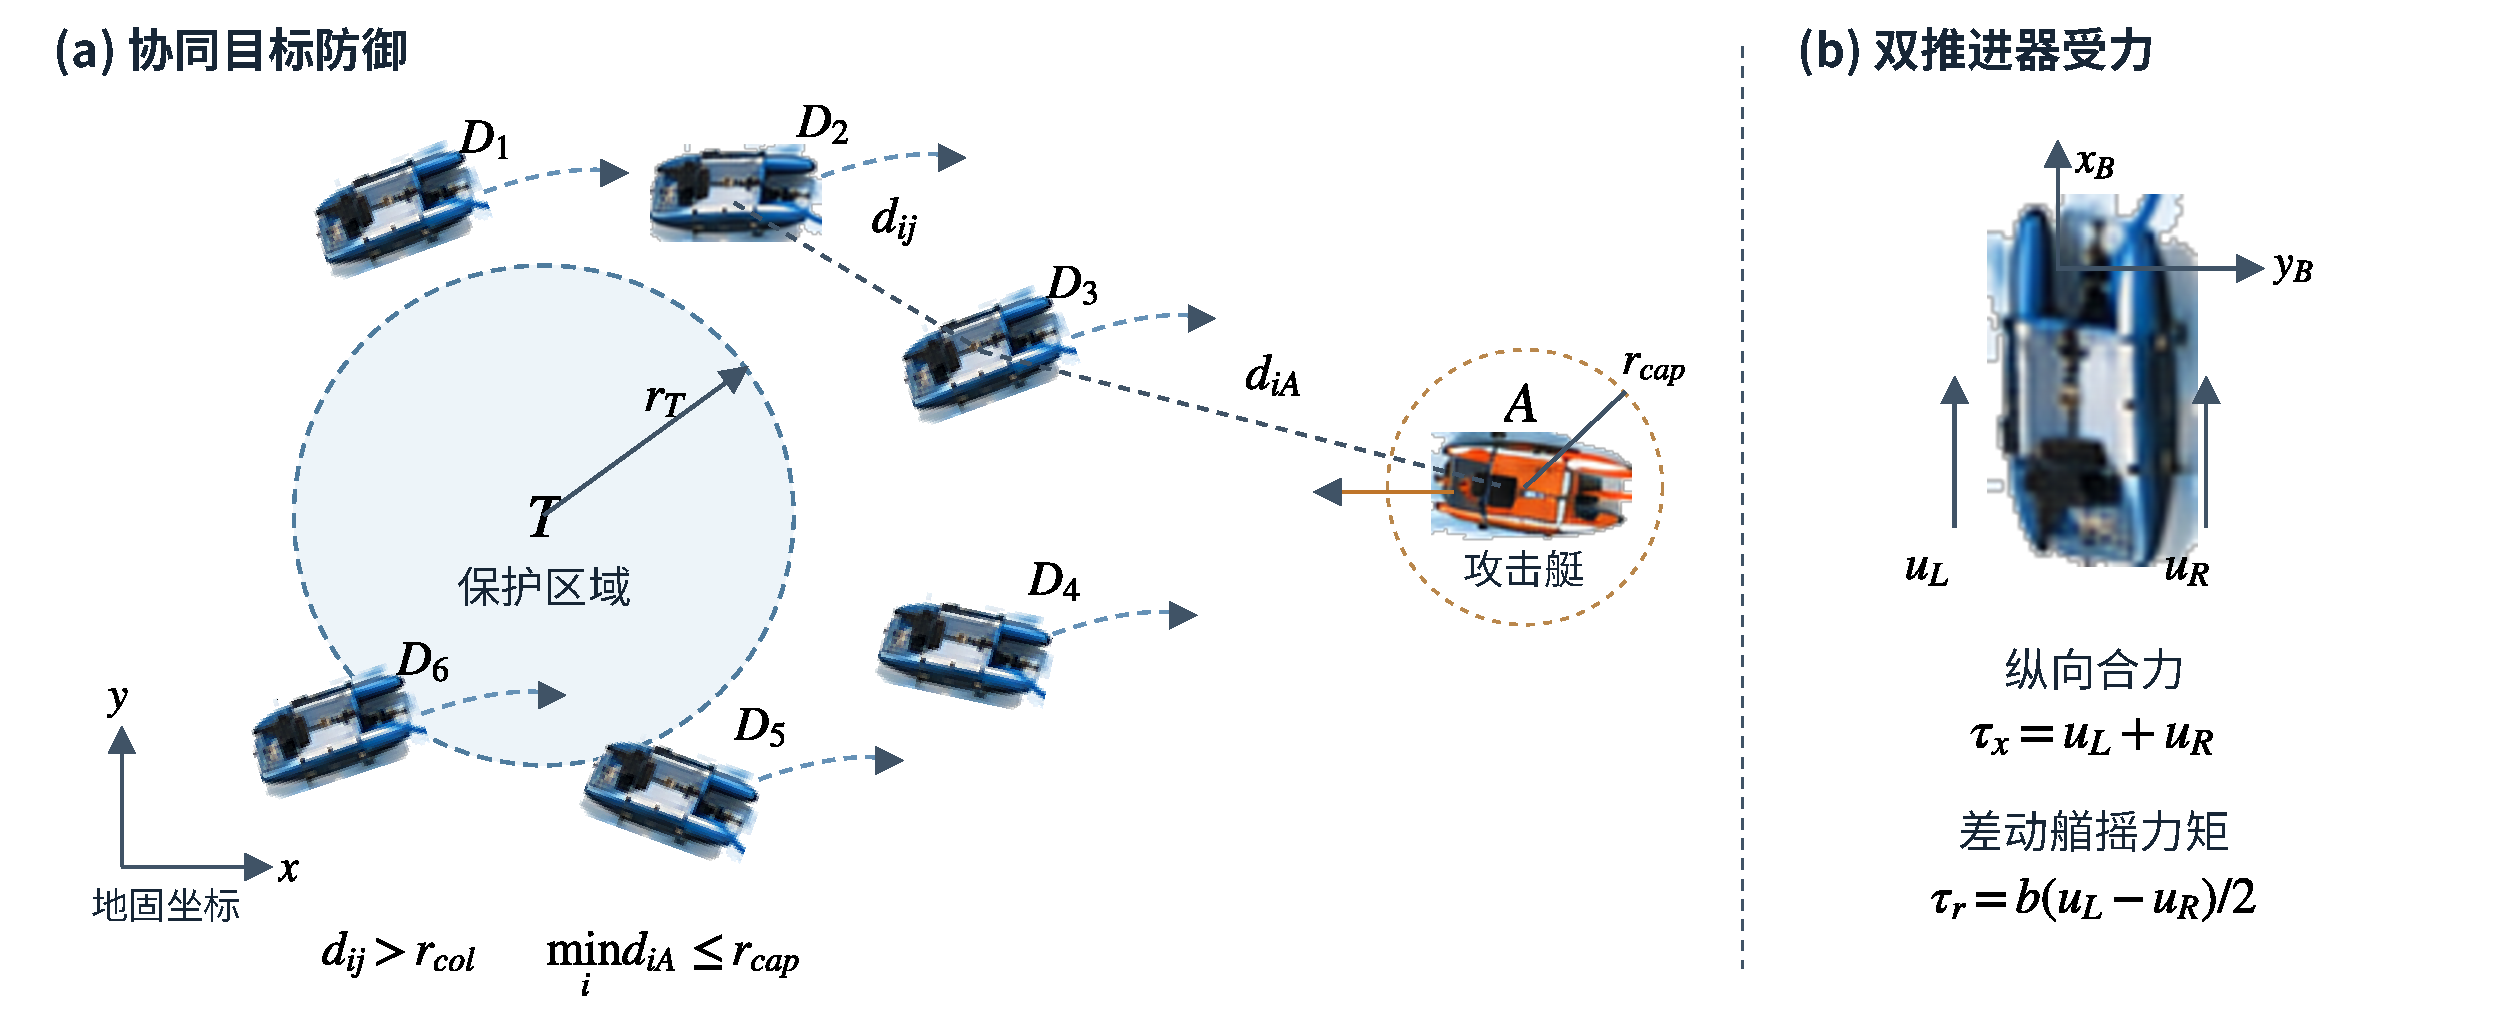
\includegraphics[width=\linewidth]{figures/fig1_task.pdf}
\caption*{图1　六艇协同目标防御及双推进器控制几何。蓝色艇为防御艇，橙色艇为攻击艇，圆形区域为保护水域。图中标示相对距离、捕获邻域及推进器合力与差动力矩。}
\end{figure}

捕获、艇间碰撞、物理突破和径向失守事件分别定义为

\[
\begin{aligned}
\mathcal C&=\{x\mid\min_i d_{iA}\leq r_{\mathrm{cap}}\},&
\mathcal F_{\mathrm{col}}&=\{x\mid\min_{i<j}d_{ij}\leq r_{\mathrm{col}}\},\\
\mathcal F_{\mathrm{br}}&=\{x\mid\|\boldsymbol p_A\|\leq r_T\},&
\mathcal F_{\mathrm{rad}}&=\{x\mid\|\boldsymbol p_A\|<\min_i\|\boldsymbol p_i\|\}.
\end{aligned}
\tag{4}
\]

径向失守对应攻击艇比全部防御艇更接近保护区中心。每个控制时刻依次检查物理突破或径向失守、艇间碰撞、捕获和任务时间终止。此前未发生失败事件而完成捕获，或持续至任务时限\(T_{\max}\)，均记为防御成功。以\(Y\in\{0,1\}\)表示终局防御结果，控制目标为

\[
\pi^\star\in\arg\max_\pi
\mathbb E_{x_0,\omega,\pi_A}[Y\mid\pi],
\qquad
\boldsymbol u_i(t)\in[u_D^{\min},u_D^{\max}]^2.
\tag{5}
\]

其中，\(x_0\)为初始任务状态，\(\omega\)为环境随机条件，\(\pi_A\)为攻击策略。当前决策状态\(x_t\)包括各艇位置、艏向和速度、源控制指令以及任务时间\(t\)，剩余时限为\(T_{\max}-t\)。源学习策略根据各艇局部观测产生动作，联合控制器汇集当前艇队状态与源控制输出，集中计算完整融合配置，各防御艇执行对应推进器指令。攻击者的后续动作由实际对抗策略根据到达状态生成。实验分别记录物理突破和径向失守，并按照上述终止顺序归类任务结局。

\section*{3
候选交互与条件价值协同融合方法}

\subsection*{3.1
推进器通道级联合融合}

CIV-RL以整队推进器融合配置为控制决策对象。设防御艇\(i\)的学习指令与规则指令分别为\(\boldsymbol u_i^L(x)\)和\(\boldsymbol u_i^B(x)\)，左右通道的融合系数为\(\boldsymbol g_i=[g_{i,L},g_{i,R}]^{\mathsf T}\in[0,1]^2\)，则实际推力为

\[
\boldsymbol u_i(x,\boldsymbol g_i)
=\boldsymbol g_i\odot\boldsymbol u_i^L(x)
+(\boldsymbol 1-\boldsymbol g_i)\odot\boldsymbol u_i^B(x).
\tag{6}
\]

\(\odot\)表示逐元素乘积。两侧推进器独立调节源指令的参与程度，整个艇队的融合配置记为\(\boldsymbol G=(\boldsymbol g_1,\ldots,\boldsymbol g_n)\)。两类源指令均满足相同推力边界时，各通道的融合结果保持在二者构成的区间内。固定当前状态与源指令，有

\[
\begin{aligned}
u_{i,a}&\in\operatorname{co}\{u_{i,a}^L,u_{i,a}^B\},\\
\delta\boldsymbol u_i
&=\operatorname{diag}(\boldsymbol u_i^L-\boldsymbol u_i^B)\,\delta\boldsymbol g_i,\\
\delta\boldsymbol\tau_i
&=B\operatorname{diag}(\boldsymbol u_i^L-\boldsymbol u_i^B)\,\delta\boldsymbol g_i.
\end{aligned}
\tag{7}
\]

因此，融合系数的控制效应同时取决于当前两类源指令。相同的系数变化在不同状态下产生不同的纵向合力与艏摇力矩变化，其后续运动又受到艇体惯性和水动力阻尼影响。当多艇同步改变融合系数时，各自的候选响应共同决定交会位置与艇间距离。CI以这些反馈响应构造联合代价，在源策略融合偏好和艇对运动关系之间确定参考配置与备选配置；CV进一步评价这些配置在完整防御过程中的终局净收益。

CI在每个推进控制周期重新计算参考策略\(\pi_0\)，CV在规定决策时刻从包含参考策略的方案集中作一次选择。非参考方案在有限作用区间内保持所选融合系数，两类源动作仍随实时状态更新，区间结束后继续采用CI反馈控制。图2给出候选生成、条件价值训练与最终推进执行之间的信息流。两项机制使用同一组融合变量，分别承担运动交互评价与长期团队结果评价。

\begin{figure}[!htbp]
\centering
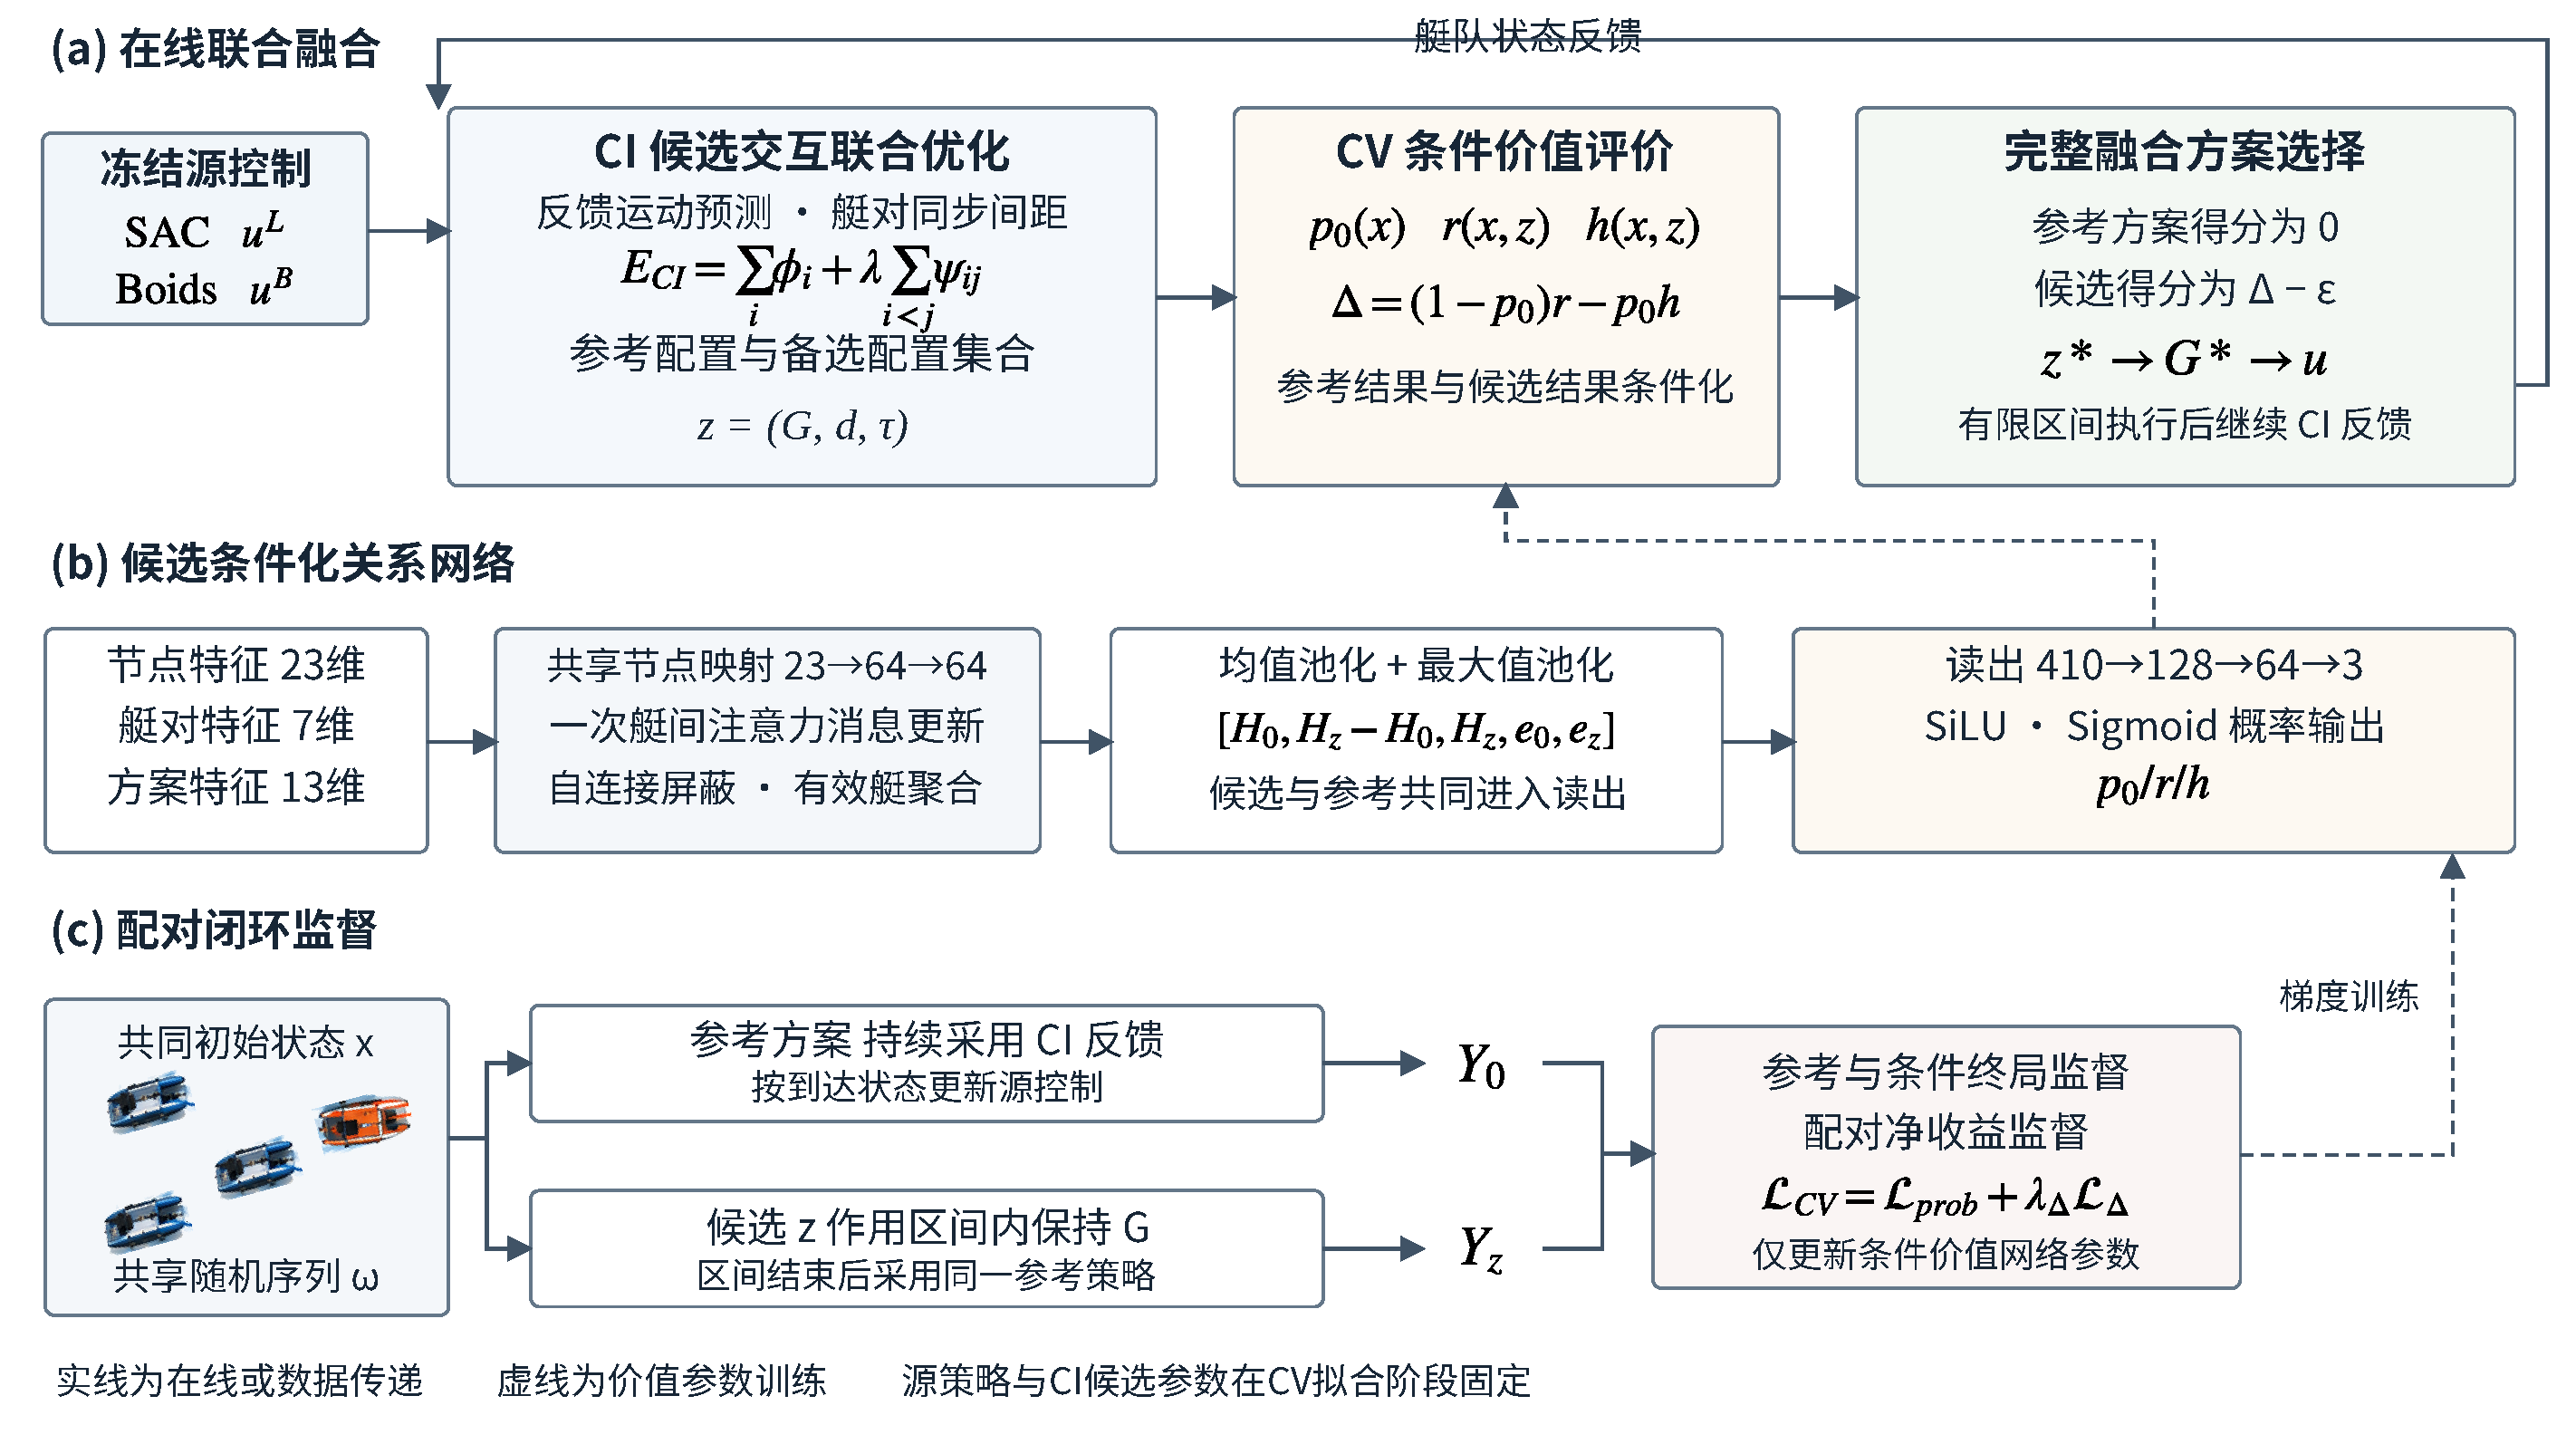
\includegraphics[width=\linewidth]{figures/fig2_architecture.pdf}
\caption*{图2　CIV-RL的联合融合与条件价值学习结构。CI依据源指令和候选反馈响应形成联合配置，CV以参考及候选的关系表示估计条件概率。实线表示在线控制，虚线表示配对终局监督与价值参数训练。}
\end{figure}

\subsection*{3.2
状态表示与源控制策略}

学习控制源采用参数共享的SAC策略{[}27{]}。各防御艇的局部观测由任务特征\(o_i^{AT}\)、群体规则特征\(o_i^B\)和队友观测集合\(\{o_{ij}\}_{j\ne i}\)组成。任务特征包含保护区和攻击艇的相对距离与方位，以及攻击艇速度的模和相对方向，共6维；每个队友以相对距离和方位表示。方位角以本艇艏向为参考并约束在\([-\pi,\pi)\)，距离保留米制量纲。Boids特征由分离、对齐、聚合作用的模与方位以及两个归一化推进器输出构成，共8维。队友观测经共享映射和均值聚合得到定长表示{[}12{]}

\[
\boldsymbol e_i^D=\frac1{|\mathcal N_i|}\sum_{j\in\mathcal N_i}f_D(o_{ij}),
\qquad
\boldsymbol h_i=f_s(o_i^{AT},\boldsymbol e_i^D,o_i^B).
\tag{8}
\]

动作网络依据\(\boldsymbol h_i\)产生学习指令，局部融合映射读取隐藏特征和两类源动作，输出标量融合偏好。源策略采用自适应融合训练形式{[}21{]}，动作网络与局部融合映射共同接受任务回报反馈。SAC的熵正则化目标为

\[
J_{\mathrm{src}}(\psi)
=\mathbb E\!\left[\sum_{k=0}^{K_T}\gamma^k
\bigl(r_k+\alpha\mathcal H(\pi_\psi(\cdot\mid o_k))\bigr)\right].
\tag{9}
\]

\(K_T\)为一回合的离散控制步数，\(\gamma\)为折扣因子，\(\alpha\)为熵温度。各同构防御艇共享参数，训练样本由艇队交互共同提供。连续动作经双曲正切约束后线性映射到推进器推力范围。局部融合输出经过有界映射形成候选中心\(\bar g_i(x)\)，并作为两侧推进器的共同中心值。

Boids控制由分离、对齐、聚合和目标吸引四类作用组成{[}7,21{]}。采用当前艇位和地固速度，实际规则场可写为

\[
\begin{aligned}
\boldsymbol F_i^{\mathrm{sep}}&=
 k_{\mathrm{sep}}\sum_{j\in\mathcal N_i^s}
 \frac{\boldsymbol p_i-\boldsymbol p_j}{\max(d_{ij}-r_b,\epsilon_b)^2},\\
\boldsymbol F_i^{\mathrm{ali}}&=\frac{k_{\mathrm{ali}}}{n}\sum_j\boldsymbol v_j,
\qquad
\boldsymbol F_i^{\mathrm{coh}}=k_{\mathrm{coh}}\left(\frac1n\sum_j\boldsymbol p_j-\boldsymbol p_i\right),\\
\boldsymbol F_i^{\mathrm{att}}&=k_{\mathrm{att}}(\boldsymbol p_A-\boldsymbol p_i),
\qquad
\boldsymbol F_i=\boldsymbol F_i^{\mathrm{sep}}+\boldsymbol F_i^{\mathrm{ali}}+
\boldsymbol F_i^{\mathrm{coh}}+\boldsymbol F_i^{\mathrm{att}}.
\end{aligned}
\tag{10}
\]

其中，\(\mathcal N_i^s=\{j\ne i\mid d_{ij}<15\,\mathrm m\}\)，\(r_b=3.5\,\mathrm m\)，\(\epsilon_b=0.01\,\mathrm m\)，四项权重依次为10、0.1、0.1和0.5。合力单位方向转换至艇体坐标后记为\(\boldsymbol f_i=[f_{x,i},f_{y,i}]^{\mathsf T}\)，方向角\(\chi_i=\operatorname{atan2}(f_{y,i},f_{x,i})\)，规则推力由

\[
\boldsymbol u_i^B=
\operatorname{clip}_{[u_D^{\min},u_D^{\max}]^2}
\left\{u_D^{\max}
\begin{bmatrix} f_{x,i}+0.75\chi_i\\ f_{x,i}-0.75\chi_i\end{bmatrix}\right\}
\tag{11}
\]

给出。源策略训练完成后，固定动作网络与局部融合映射。学习动作和规则动作提供候选控制端点，局部融合输出提供候选中心，CI负责候选组合的联合选择，CV负责对应完整方案的任务价值评价。

\subsection*{3.3
候选反馈响应与联合配置优化}

防御艇\(i\)的候选集合记为\(\mathcal G_i(x)=\{\boldsymbol g_i^1,\ldots,\boldsymbol g_i^{K_i}\}\)，由规则端点、学习端点和源策略融合中心的通道组合\(\{0,\bar g_i(x),1\}^2\)生成，每艇至多具有9个不同候选。将重合系数组合合并后，候选相对于源策略偏好的局部代价定义为

\[
\phi_i(k;x)=\frac12\sum_{a\in\{L,R\}}
\left(\frac{g_{i,a}^{k}-\bar g_i(x)}{\sigma_g}\right)^2.
\tag{12}
\]

\(\sigma_g\)为偏离尺度。该项在候选选择中保留源策略通过任务训练形成的机动偏好。CI进一步预测每个候选的运动响应，比较不同艇的候选共同执行时的同步接近关系。

预测以当前艇队状态为起点，在时域\(H\)内保持候选融合系数。其他防御艇和攻击艇的名义位置按当前地固速度延续

\[
\widehat{\boldsymbol p}^{\mathrm{nom}}_j(s)
=\boldsymbol p_j+s\boldsymbol v_j,
\qquad
\widehat{\boldsymbol p}^{\mathrm{nom}}_A(s)
=\boldsymbol p_A+s\boldsymbol v_A,
\qquad s\in[0,H].
\tag{13}
\]

各候选共享上述名义运动条件。设\(\widehat x_{i,q}^{k}\)为艇\(i\)执行第\(k\)个候选时的预测状态，\(\widehat o_{i,q}^{k}\)为根据本艇预测状态、其他艇名义运动和攻击艇名义运动构造的局部观测。候选反馈递推为

\[
\begin{aligned}
\widehat o_{i,q}^{k}
&=\mathcal O_i\!\left(\widehat x_{i,q}^{k},
\widehat{\boldsymbol x}_{-i,q}^{\mathrm{nom}},\widehat x_{A,q}^{\mathrm{nom}}\right),\\
\widehat{\boldsymbol u}_{i,q}^{k}
&=\boldsymbol g_i^k\odot\pi_L(\widehat o_{i,q}^{k})
+(\boldsymbol1-\boldsymbol g_i^k)\odot\pi_B(\widehat o_{i,q}^{k}),\\
\widehat x_{i,q+1}^{k}
&=\widehat F\!\left(\widehat x_{i,q}^{k},\widehat{\boldsymbol u}_{i,q}^{k}\right),
\qquad \widehat x_{i,0}^{k}=x_i.
\end{aligned}
\tag{14}
\]

\(\mathcal O_i\)沿用源策略观测定义，\(\widehat F\)为平面动力学离散转移。名义邻艇轨迹参与观测与规则场的计算，本艇源指令随预测状态重新生成。本文预测步长为0.1
s，源指令每0.2 s刷新，预测时域为3.2
s。候选位置序列记为\(\widehat{\boldsymbol p}_i^k(s_q)\)，其中\(s_q=q\Delta t_{\mathrm{pred}}\)。对艇\(i\)和\(j\)的候选组合\((k,\ell)\)，定义

\[
\begin{aligned}
d_{ij}^{k\ell}(x)
&=\min_{q=1,\ldots,N_H}
\left\|\widehat{\boldsymbol p}_i^k(s_q)-\widehat{\boldsymbol p}_j^\ell(s_q)\right\|,\\
\psi_{ij}(k,\ell;x)&=\left[r_s-d_{ij}^{k\ell}(x)\right]_+^2,
\qquad N_H=H/\Delta t_{\mathrm{pred}}.
\end{aligned}
\tag{15}
\]

\(r_s\)为候选接近评价距离，\([a]_+=\max(a,0)\)。最小间距在同步离散预测时刻计算，交互势因而描述两个候选同时执行时的近距交会。同一艘艇的候选在不同队友选择下具有不同代价，图3(a)给出相应的几何关系。

以\(\boldsymbol k=(k_1,\ldots,k_n)\)表示艇队候选索引，联合融合目标写为

\[
\begin{aligned}
E_{\mathrm{CI}}(x,\boldsymbol k)
&=\sum_{i=1}^{n}\phi_i(k_i;x)
+\lambda\sum_{i<j}\psi_{ij}(k_i,k_j;x),\\
\boldsymbol k^\star&\in\arg\min_{\boldsymbol k\in\prod_i\{1,\ldots,K_i\}}
E_{\mathrm{CI}}(x,\boldsymbol k).
\end{aligned}
\tag{16}
\]

\(\lambda\)为交互权重，\(\boldsymbol k^\star\)表示目标最优配置。有限搜索得到参考索引\(\boldsymbol k_0\)及相应融合配置\(\boldsymbol G_0(x)\)。局部代价保持源策略的融合偏好，艇对项评价双方实际候选组合的接近程度。在保持其余艇选择不变时，艇\(i\)由\(k_i\)调整为\(k_i'\)引起的目标变化为

\[
\delta E_i=
\phi_i(k_i';x)-\phi_i(k_i;x)
+\lambda\sum_{j\ne i}
\left[\psi_{ij}(k_i',k_j;x)-\psi_{ij}(k_i,k_j;x)\right].
\tag{17}
\]

式（17）中的交互变化由队友实际选定的\(k_j\)决定。联合求解据此在整队配置上调整相互接近的候选组合，同时维持源策略的任务机动偏好。

配置求解采用束搜索和局部细化。束搜索依次扩展各艇候选，累计新增局部代价及其与已选候选的艇对代价，每轮保留能量最低的有限个部分配置，获得联合目标的有限搜索近似解。完整配置形成后执行三轮坐标更新，并在保留配置上进行一次双艇块细化。与原参考配置相比，采用的细化结果同时满足局部偏离总量和预测交互总量均不增加。每艇候选数上限为9时，完整组合数为\(9^n\)，预先计算的不同艇对代价至多包含\(81n(n-1)/2\)项；受限束宽控制完整配置搜索的规模，局部更新重复使用同一艇对代价表。

参考配置、保留的搜索结果和参考配置的单艇邻域构成候选池\(\mathcal P(x)\)。在给定能量容差下，备选配置集合为

\[
\mathcal C(x)=\{\boldsymbol G_0(x)\}\cup
\left\{\boldsymbol G\in\mathcal P(x)\ \middle|\
E_{\mathrm{CI}}(x,\boldsymbol G)
\leq E_{\mathrm{CI}}(x,\boldsymbol G_0)+n\rho\right\}.
\tag{18}
\]

其中，\(\rho\)为单位艇数的代价容差。集合内去除重复配置，并按联合能量保留规定数量的备选。CI在每个控制周期求得参考配置，CV在规定时刻进一步评价备选配置的完整任务后果。

\begin{figure}[!htbp]
\centering
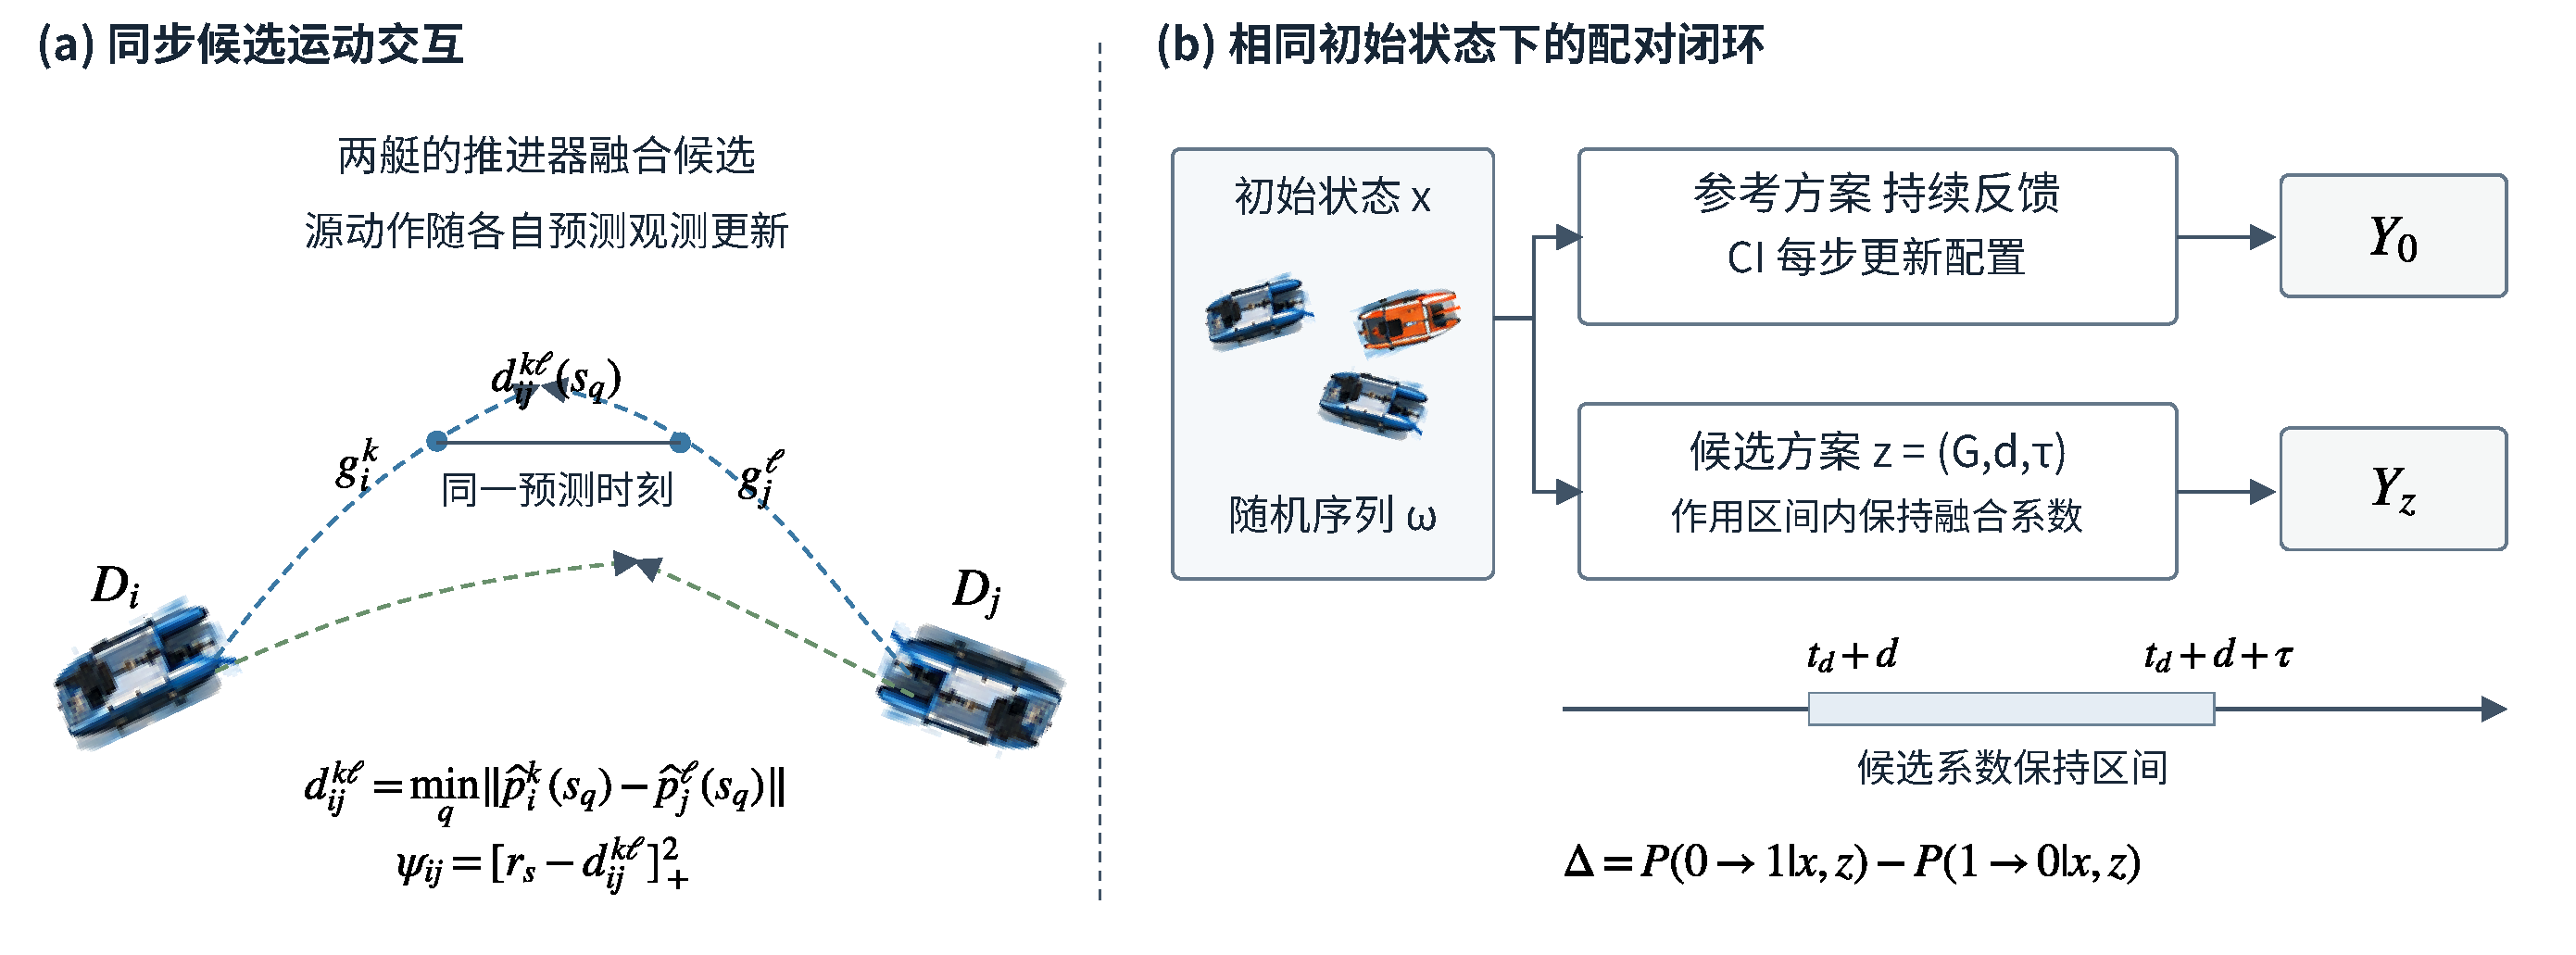
\includegraphics[width=\linewidth]{figures/fig3_mechanisms.pdf}
\caption*{图3　候选运动与配对闭环条件价值。（a）两艇候选在同步预测时刻的接近关系，最小间距由同一时间索引下的预测位置确定。（b）参考反馈方案与有限作用候选方案共享初始状态及随机序列，各分支独立反馈执行至终局。}
\end{figure}

\subsection*{3.4
完整融合方案与配对条件价值}

完整方案\(z=(\boldsymbol G,d,\tau)\)由融合配置、执行延迟和作用时长组成。参考方案\(z_0\)持续执行每步更新的CI策略\(\pi_0\)。设方案决策时刻为\(t_d\)，候选在\([t_d+d,t_d+d+\tau)\)内保持指定系数，其余时刻执行参考策略

\[
\boldsymbol g_i(t;z)=
\begin{cases}
\boldsymbol g_i^z,&t_d+d\leq t<t_d+d+\tau,\\
\boldsymbol g_i^0(x_t),&\text{其余时刻}.
\end{cases}
\tag{19}
\]

源学习指令和Boids指令在各分支的当前状态上持续更新。令\(\mathcal D\)和\(\mathcal T_\tau\)分别为允许的延迟与作用时长集合，当前候选方案集为

\[
\mathcal Z_{\mathrm{CI}}(x)=\{z_0\}\cup
\left\{(\boldsymbol G,d,\tau)\ \middle|\
\boldsymbol G\in\mathcal C(x)\setminus\{\boldsymbol G_0(x)\},\
d\in\mathcal D,\ \tau\in\mathcal T_\tau\right\}.
\tag{20}
\]

\(z_0\)对应持续重求CI配置的反馈过程，候选对应指定系数在有限区间内的保持过程。当前方案集中仅将非参考配置与作用时长组合，参考配置通过\(z_0\)进入最终选择。配置池与时序集合由此共同规定CV实际评价的控制过程。

将配对闭环推演的初始状态记为\(x\)，共同随机序列记为\(\omega\)。在相同参考策略参数下，方案\(z\)的终局结果及条件价值定义为

\[
Y(x,z,\omega)=\mathbb I\{\text{闭环防御成功}\},
\qquad
V^{\pi_0}(x,z)=\mathbb E_\omega[Y(x,z,\omega)].
\tag{21}
\]

参考与候选分支共享\(x\)和\(\omega\)，随后依据各自到达的状态重新计算控制。若两个方案具有相同作用区间，且仅在一艘艇的融合系数上不同，则构成局部融合比较，其余艇的当前配置保持一致。以\(R_x\)组共同随机序列进行完整续行，经验条件价值差为

\[
\widehat\Delta(x;z,z')
=\frac1{R_x}\sum_{q=1}^{R_x}
\left[Y(x,z',\omega_q)-Y(x,z,\omega_q)\right].
\tag{22}
\]

单艇变化比较和多艇配置比较均使用完整团队终局结果。CV以共享函数\(V_\theta(x,z)\)表示方案价值，任意两个方案的预测差为

\[
\Delta_\theta(x;z,z')=V_\theta(x,z')-V_\theta(x,z).
\tag{23}
\]

记\(Y_0=Y(x,z_0,\omega)\)和\(Y_z=Y(x,z,\omega)\)。参考方案与候选方案具有相同结果的配对样本对净成功变化的贡献为零，相对收益由两类成败转化确定

\[
\Delta(x;z_0,z)
=\Pr(Y_0=0,Y_z=1\mid x,z)
-\Pr(Y_0=1,Y_z=0\mid x,z).
\tag{24}
\]

据此定义参考成功概率、参考失败时的候选成功概率和参考成功时的候选失败概率

\[
\begin{aligned}
p_{0,\theta}(x)&=\Pr(Y_0=1\mid x),\\
r_\theta(x,z)&=\Pr(Y_z=1\mid Y_0=0,x,z),\\
h_\theta(x,z)&=\Pr(Y_z=0\mid Y_0=1,x,z).
\end{aligned}
\tag{25}
\]

条件模型得到的完整方案价值与相对参考收益为

\[
\begin{aligned}
V_\theta(x,z)
&=[1-p_{0,\theta}(x)]r_\theta(x,z)
+p_{0,\theta}(x)[1-h_\theta(x,z)],\\
\Delta_\theta(x;z_0,z)
&=[1-p_{0,\theta}(x)]r_\theta(x,z)
-p_{0,\theta}(x)h_\theta(x,z),\\
V_\theta(x,z_0)&=p_{0,\theta}(x).
\end{aligned}
\tag{26}
\]

\(r_\theta\)学习参考失败时的成功恢复机会，\(h_\theta\)学习改变原有成功结果的概率，二者按照参考结果的发生概率组合为净收益。与直接拟合候选终局成功率相比，该表示保留了候选结果所对应的参考事件。条件价值的学习和最终方案选择因此使用同一成败转化量，式（23）进一步将局部变化和完整配置比较归于共同价值基准。

\subsection*{3.5
候选条件化的关系表示与监督训练}

条件价值网络以当前艇队状态与完整候选方案为输入。节点特征\(\boldsymbol\xi_i(x,z)\in\mathbb R^{23}\)包含本艇相对于攻击艇的位置和速度、艏向方向、角速度、规则与学习指令、参考和候选融合系数、系数差、参考和候选预测位移以及局部代价和交互统计。艇对特征\(\boldsymbol\rho_{ij}(x,z)\in\mathbb R^7\)包含相对位置、相对速度、候选预测终点差和艇对交互势。方案级特征\(\boldsymbol e_z\in\mathbb R^{13}\)包含攻击艇至保护区的距离和运动方向、艇数、任务时间、联合代价统计、候选来源标记及作用区间。关系坐标以攻击艇指向保护区的方向为基轴，位置和速度分别按30
m与5 m/s缩放，地固方位信息保留在方案级输入中。

节点表示随候选系数和预测运动变化，同一艇队状态下的不同融合配置形成不同关系表示。共享节点映射后进行一次注意力消息聚合

\[
\begin{aligned}
\boldsymbol h_i&=f_n(\boldsymbol\xi_i),\\
a_{ij}&=\frac{\exp f_a(\boldsymbol h_i,\boldsymbol h_j,\boldsymbol\rho_{ij})}
{\sum_{k\ne i}\exp f_a(\boldsymbol h_i,\boldsymbol h_k,\boldsymbol\rho_{ik})},
\qquad j\ne i,\\
\boldsymbol h_i^+&=f_u\!\left(\boldsymbol h_i,
\sum_{j\ne i}a_{ij}f_m(\boldsymbol h_i,\boldsymbol h_j,\boldsymbol\rho_{ij})\right).
\end{aligned}
\tag{27}
\]

注意力屏蔽自连接，消息仅在当前有效防御艇之间传递。对更新后的节点进行均值和最大值聚合，形成方案表示\(\boldsymbol H_z\)。读出层同时使用参考表示、候选表示及其差异

\[
\begin{aligned}
\boldsymbol H_z&=\left[\operatorname{Mean}_i\boldsymbol h_i^+,
\operatorname{Max}_i\boldsymbol h_i^+\right],\\
\boldsymbol\ell_\theta(x,z)
&=f_o\!\left(\boldsymbol H_{z_0},\boldsymbol H_z-\boldsymbol H_{z_0},
\boldsymbol H_z,\boldsymbol e_{z_0},\boldsymbol e_z\right).
\end{aligned}
\tag{28}
\]

节点映射为两层64维全连接网络，消息映射采用\(135\!\rightarrow\!64\!\rightarrow\!64\)结构，注意力映射采用\(135\!\rightarrow\!32\!\rightarrow\!1\)结构，节点更新采用\(128\!\rightarrow\!64\!\rightarrow\!64\)结构。均值与最大值聚合产生128维方案表示，读出输入为410维，经128维和64维隐藏层输出三个标量。隐藏层采用SiLU激活，读出层训练时使用0.04的随机失活率。参考方案的第一输出经Sigmoid映射形成\(p_{0,\theta}\)，候选的另两项输出形成\(r_\theta\)与\(h_\theta\)。训练样本确定输入的均值和尺度，验证及执行保持相同标准化参数。不同艇数通过共享映射和当前艇集合上的聚合处理，无效候选由掩码排除。

训练同时使用参考终局监督、条件终局监督和配对收益监督。设\(\ell(p,y)=-y\log p-(1-y)\log(1-p)\)，概率目标写为

\[
\mathcal L_{\mathrm{prob}}
=\mathbb E_{\mathcal D}^{\iota}\ell(p_{0,\theta},Y_0)
+\frac12\mathbb E_{\mathcal D\mid Y_0=0}^{\iota,m}\ell(r_\theta,Y_z)
+\frac12\mathbb E_{\mathcal D\mid Y_0=1}^{\iota,m}\ell(h_\theta,1-Y_z).
\tag{29}
\]

其中，\(\iota_x\)为初始状态的采样校正权重，\(m_{xz}\)为候选有效掩码。参考概率项对抽样批次作加权平均，两个条件项分别在对应参考事件下按有效样本权重之和归一化。参考终局标签确定当前CI策略的成功水平，条件标签分别拟合候选在参考失败与成功事件下的结果分布。

对同一初始状态和候选，将共同随机序列下的终局差平均为\(\bar\delta_{xz}=R_x^{-1}\sum_q(Y_z^{(q)}-Y_0^{(q)})\)。配对收益监督对参考概率分支采用梯度截断

\[
\widetilde\Delta_\theta(x,z)
=[1-\operatorname{sg}(p_{0,\theta}(x))]r_\theta(x,z)
-\operatorname{sg}(p_{0,\theta}(x))h_\theta(x,z),
\tag{30}
\]

并构造

\[
\begin{aligned}
\mathcal L_\Delta
&=\frac{\displaystyle\sum_{x,z\ne z_0}w_{xz}
[\widetilde\Delta_\theta(x,z)-\bar\delta_{xz}]^2}
{\displaystyle\sum_{x,z\ne z_0}w_{xz}},\\
w_{xz}&=\iota_xm_{xz}(1+3|\bar\delta_{xz}|),
\qquad
\mathcal L_{\mathrm{CV}}=\mathcal L_{\mathrm{prob}}+\lambda_\Delta\mathcal L_\Delta.
\end{aligned}
\tag{31}
\]

配对项直接约束最终用于方案选择的净收益估计，其显式差值梯度作用于条件结果估计，参考概率保留终局交叉熵监督。模型对初始状态进行自助重采样，并依据实际采样概率校正权重。源策略和CI候选生成参数在条件价值训练阶段固定，多个模型成员分别完成拟合，执行时平均成员给出的候选净收益。

\subsection*{3.6
条件价值引导的融合方案选择}

CV对CI提供的联合配置及其作用时长进行评价，将参考方案的相对收益设为零。以\(\overline\Delta_\theta(x,z)\)表示模型成员的平均预测收益，\(\varepsilon\)为接受阈值，最终评分及方案选择为

\[
S_\theta(x,z)=
\begin{cases}
0,&z=z_0,\\
\overline\Delta_\theta(x,z)-\varepsilon,&z\ne z_0,
\end{cases}
\qquad
z^\star\in\arg\max_{z\in\mathcal Z_{\mathrm{CI}}(x)}S_\theta(x,z).
\tag{32}
\]

最高分为零时保留参考方案。候选被接受后，所选融合系数按式（19）作用于实时源指令

\[
\boldsymbol u_i(t)
=\boldsymbol g_i(t;z^\star)\odot\boldsymbol u_i^L(x_t)
+[\boldsymbol1-\boldsymbol g_i(t;z^\star)]\odot\boldsymbol u_i^B(x_t).
\tag{33}
\]

CI的交互代价通过候选构造与能量筛选限制可选配置，CV的终局价值通过式（32）决定是否采用相应候选。在作用区间内，艇队持续获得状态反馈，学习指令和规则指令随状态变化；区间结束后，CI继续逐步求解参考配置。配对训练与在线控制使用相同的作用区间和后续策略。

式（26）还给出预测收益的自然边界。由于三个输出均属于\([0,1]\)，单个模型成员满足

\[
-p_{0,\theta}(x)\leq\Delta_\theta(x;z_0,z)\leq1-p_{0,\theta}(x).
\tag{34}
\]

平均成员预测后，收益上界为\(1-\bar p_0(x)\)。按照严格正得分接受规则，当\(\bar p_0(x)\geq1-\varepsilon\)时，所有候选均保留在参考方案以下或与其并列，控制器执行\(z_0\)。参考成功水平由此直接影响候选改变可获得的预测增益范围。当前\(\varepsilon=0.075\)对应界值0.925。

本文在\(t_d=4\)
s进行一次方案选择，\(\mathcal D=\{0\}\)，\(\mathcal T_\tau=\{1\,\mathrm s,4\,\mathrm s\}\)。CI在0.2
s控制周期内持续更新，CV仅在规定决策时刻评价有效候选。其执行过程依次包括源指令生成、候选反馈预测、联合配置求解、条件净收益排序和通道融合，选择参考时直接沿用当前CI反馈配置。

\subsection*{3.7
奖励与训练过程}

源策略依据逐步任务奖励学习推进控制与局部融合偏好，条件价值模型依据配对终局标签学习完整方案的成功概率和相对收益。源训练沿用任务反馈、队形反馈与碰撞反馈的组合{[}21{]}

\[
r_i=r_i^{\mathrm{task}}+r_i^{\mathrm{form}}+r_i^{\mathrm{col}}.
\tag{35}
\]

任务项在攻击者突破或径向失守时施加失败反馈，在完成捕获时向捕获艇及其近邻协助艇提供奖励。协助邻域由\(3r_{\mathrm{cap}}\)确定。碰撞项依据发生近距接触的艇对施加惩罚。队形项将防御艇相对于攻击艇的方向与保护区的受威胁方向联系起来，定义

\[
\begin{aligned}
\widehat{\boldsymbol d}_{iA}
&=\frac{\boldsymbol p_A-\boldsymbol p_i}{\|\boldsymbol p_A-\boldsymbol p_i\|},
\quad
\boldsymbol d_{DA}=\sum_i\widehat{\boldsymbol d}_{iA},
\quad
\widehat{\boldsymbol d}_{TA}=\frac{\boldsymbol p_A}{\|\boldsymbol p_A\|},\\
r_i^{\mathrm{form}}
&=0.5\widehat{\boldsymbol d}_{TA}^{\mathsf T}
\frac{\boldsymbol d_{DA}}{\|\boldsymbol d_{DA}\|}
-\frac{\|\boldsymbol d_{DA}\|}{n}.
\end{aligned}
\tag{36}
\]

零范数时相应方向项取零。方向项评价艇队相对于攻击方向的拦截分布，合向量模长项约束各艇接近方向的集中程度。

源策略采用攻击者机动性课程{[}28{]}，平均难度随训练推进提高，每回合从以平均机动系数\(\bar L_{\mathrm{agi}}(k)\)为中心的区间中采样

\[
L_{\mathrm{agi}}\sim\mathcal U\!\left(
\bar L_{\mathrm{agi}}(k)-\delta_L,
\bar L_{\mathrm{agi}}(k)+\delta_L\right).
\tag{37}
\]

\(k\)为源训练环境交互步数，\(K_c\)为课程更新间隔，\(L_0\)、\(\Delta L\)和\(\delta_L\)分别为初始难度、增长量和采样半宽。训练依次完成源策略学习、固定控制源下的配对闭环采集和条件价值拟合。前一阶段的逐步回报塑造源动作与局部融合偏好，后一阶段的二元终局标签评价同一候选空间中的完整方案。源训练的奖励系数和课程记录列于表1，条件价值训练使用式（31），两个阶段的反馈与参数更新分别定义。

\FloatBarrier\section*{4 实验与分析}

\subsection*{4.1 实验设置}

数值评价采用六艘防御艇对单艘攻击艇的区域防御任务。保护区域半径为15
m，捕获距离与艇间碰撞距离均为5 m，任务时限为80 s。动力学积分周期为0.05
s，推进器控制周期为0.2 s，单推进器推力范围为\([-500,1000]\)
N。攻击艇采用由保护区域吸引与防御艇排斥形成的人工势场策略。主评价包含\(L_{\mathrm{agi}}=2.0\)和2.5两种条件，各100个任务。

初始防御艇分布在距目标中心7至8
m的圆周附近，以随机初始方位和等间隔角度布设，各艇艏向在共同随机方向上叠加\([-\pi/3,\pi/3]\)的偏差。攻击艇初始距离在60至65
m内采样，来向覆盖完整方位范围。所有方法在相同位置、航向、机动条件和随机序列下配对评价。源控制在每个分支的实时观测上计算，数值试验与高保真试验分别记录各自的实际控制过程。

CI预测时域为3.2 s，预测步长为0.1
s，局部偏好尺度为0.4，交互权重为32，候选接近评价距离为7
m。联合搜索束宽为128，参考与备选配置总数上限为6，单位艇数能量容差为0.5。CV在4
s进行单次决策，执行延迟为零，作用时长为1 s或4
s，故包含参考方案在内至多评价11个有效方案。接受阈值在开发任务中确定为0.075，冻结后用于正式评价。

源学习策略在六艇环境中完成\(10^6\)步交互。条件价值训练使用772个配对初始状态，验证使用206个状态，同一场景及其共同随机续行始终归入同一数据划分。采集条件覆盖机动系数2.0、2.5、3.0和3.5。每个状态的配对随机条件数为1、2、5或6，训练与验证分别包含16
544条和3
575条有效终局观测。三个关系网络成员采用独立初始状态自助采样，每个成员有96
420个可训练参数。训练上限为每成员4 500次更新，条件价值模型选用每成员1
500次更新的检查点，普通价值对照选用每成员4
500次更新的检查点。两者共享控制源、关系网络、候选方案、训练样本及最大更新预算。模型采用AdamW优化，学习率为\(3\times10^{-4}\)，批量大小为48，权重衰减为\(10^{-4}\)。主要设置见表1。

\Needspace{10\baselineskip}
\begin{center}\small\bfseries 表1　任务、控制与学习参数\end{center}

\begingroup
\small
\setlength{\tabcolsep}{3.2pt}
\begin{longtable}{@{}>{\raggedright\arraybackslash}p{(\linewidth - 4\tabcolsep) * \real{0.42}}
>{\raggedright\arraybackslash}p{(\linewidth - 4\tabcolsep) * \real{0.22}}
>{\raggedright\arraybackslash}p{(\linewidth - 4\tabcolsep) * \real{0.36}}@{}}
\toprule\noalign{}
\begin{minipage}[b]{\linewidth}\raggedright
参数
\end{minipage} & \begin{minipage}[b]{\linewidth}\raggedright
符号
\end{minipage} & \begin{minipage}[b]{\linewidth}\raggedright
设置
\end{minipage} \\
\midrule\noalign{}
\endhead
\bottomrule\noalign{}
\endlastfoot
主任务防御艇数量 & \(n\) & 6 \\
任务时限 & \(T_{\max}\) & 80 s \\
控制周期与积分周期 & \(\Delta t,\Delta t_{\mathrm{int}}\) & 0.2 s，0.05
s \\
保护区域半径 & \(r_T\) & 15 m \\
数值捕获与碰撞阈值 & \(r_{\mathrm{cap}},r_{\mathrm{col}}\) & 5 m，5 m \\
单推进器推力范围 & \([u_D^{\min},u_D^{\max}]\) & \([-500,1000]\) N \\
CI预测时域与步长 & \(H,\Delta t_{\mathrm{pred}}\) & 3.2 s，0.1 s \\
候选接近评价距离 & \(r_s\) & 7 m \\
源策略偏好尺度与交互权重 & \(\sigma_g,\lambda\) & 0.4，32 \\
联合搜索束宽 & \(B_s\) & 128 \\
配置数上限与代价容差 & \(K_G,\rho\) & 6，0.5 \\
CV决策时刻与执行延迟 & \(t_d,d\) & 4 s，0 s \\
候选作用时长与接受阈值 & \(\tau,\varepsilon\) & 1 s或4 s，0.075 \\
训练与验证初始状态数 & \(N_{\mathrm{tr}},N_{\mathrm{val}}\) &
772，206 \\
训练与验证终局观测数 & & 16 544，3 575 \\
节点、艇对与方案特征维数 & & 23，7，13 \\
隐藏维数与消息更新次数 & & 64，1 \\
价值网络成员数与单成员参数数 & & 3，96 420 \\
最大更新次数与选定CV更新次数 & & 4 500，1 500，均按成员计 \\
配对收益权重 & \(\lambda_\Delta\) & 2 \\
源策略环境交互步数 & \(N_{\mathrm{src}}\) & \(10^6\) \\
源奖励系数 & & ［　］ \\
课程起点、增长量及更新间隔 & \(L_0,\Delta L,K_c\) & ［　］ \\
机动性采样半宽 & \(\delta_L\) & ［　］ \\
数值主评价任务数 & \(N\) & 200 \\
推理设备 & & NVIDIA GeForce RTX 4090 \\
\end{longtable}
\endgroup

当前主评价使用各方法对应的一个冻结训练流程，成功比例给出Wilson
95\%置信区间。独立完整训练的运行数、均值和标准差保留于补充表S2。对于相同的\(N\)个任务，方法\(\pi\)相对参考\(\pi_b\)的配对成功率差为

\[
\widehat\delta_{\mathrm{SR}}(\pi,\pi_b)
=\frac1N\sum_{e=1}^N\left(Y_e^\pi-Y_e^{\pi_b}\right)
=\frac{N_{01}-N_{10}}N.
\tag{38}
\]

\(N_{01}\)为参考失败而被比较方法成功的任务数，\(N_{10}\)为参考成功而被比较方法失败的任务数。任务级区间按共同场景统计，训练运行间差异按完整训练流程统计。捕获时间在成功捕获回合内求平均，对两种方法均捕获的任务另行计算配对时间差。实验同时记录捕获、艇间碰撞、径向失守、物理突破和时间终止。源策略交互、配对闭环采集及价值网络拟合分别计量，在线时延包含候选预测、联合求解和价值选择。

\subsection*{4.2
高保真闭环防御}

高保真试验在Gazebo
VRX水面环境中运行WAM-V防御艇与攻击艇。完整CIV-RL、仅CI和ARBoids使用共同初始位置、双推进器控制形式及0.2
s控制周期。任务时限为80 s，保护区域半径为15 m，艇间碰撞阈值为5
m，捕获阈值为5.5
m。12组共同场景形成36次有效闭环任务。图4展示首个配对场景的实际仿真画面，以及同一任务在接近、方案选择和捕获阶段的记录轨迹。

\begin{figure}[!htbp]
\centering
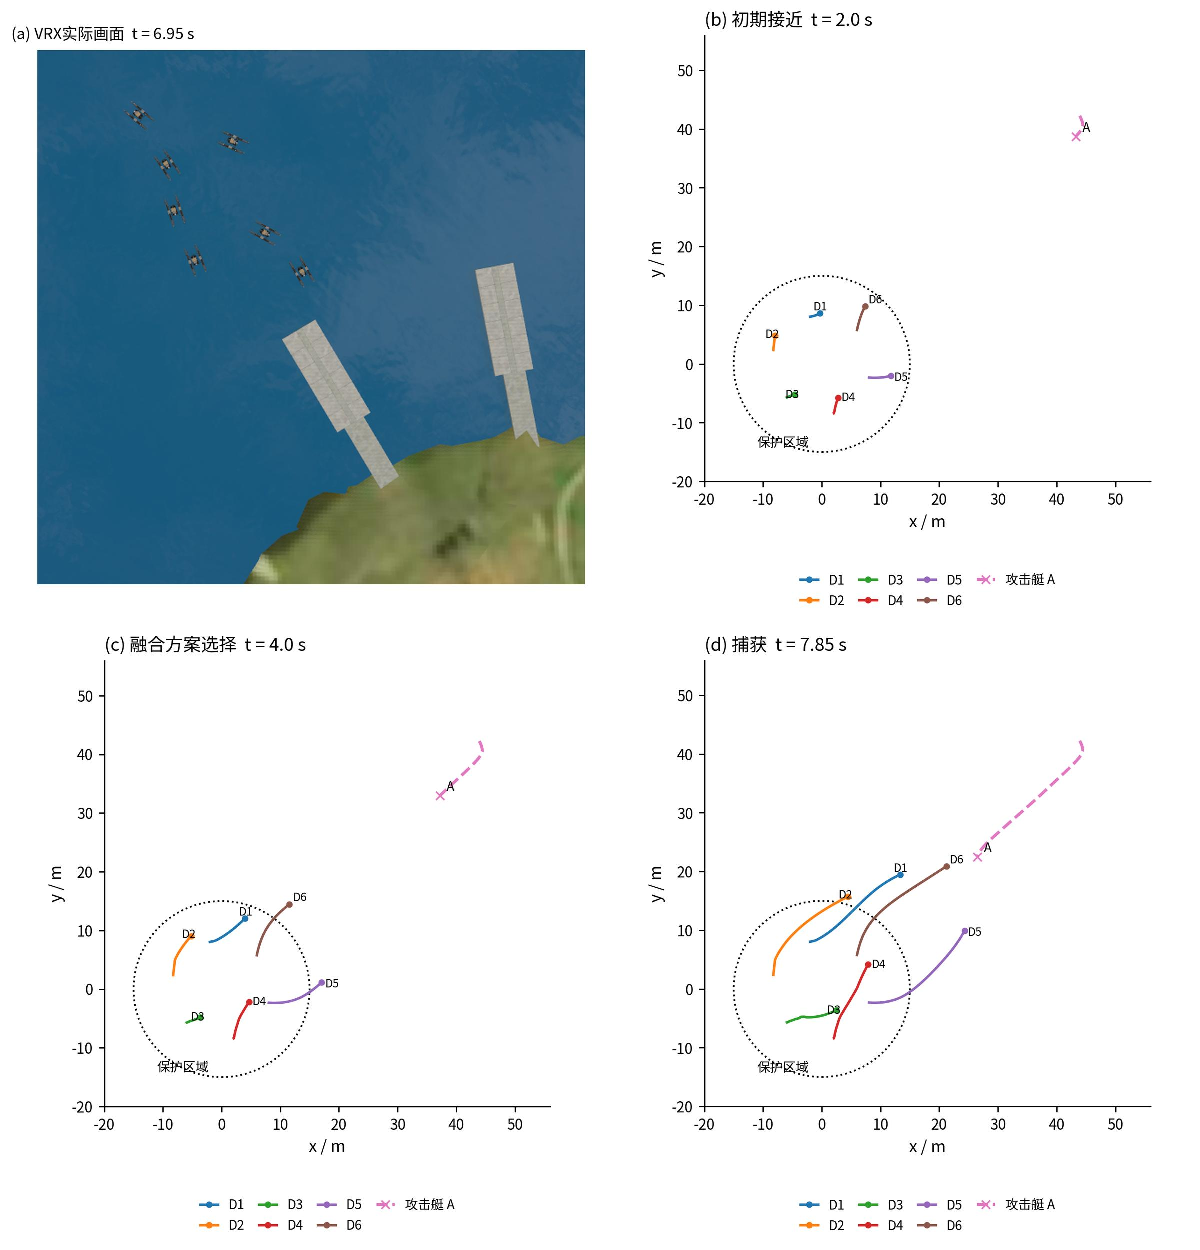
\includegraphics[width=\linewidth]{figures/fig4_vrx.pdf}
\caption*{图4　VRX协同防御过程。（a）6.95 s时的真实仿真画面。（b）2.0
s的初期接近轨迹。（c）4.0 s的艇队运动状态。（d）7.85
s捕获时的完整轨迹。轨迹阶段由同一任务记录截取，终点使用实际终止位置。}
\end{figure}

在该场景中，攻击艇由保护区域东北侧进入，防御艇沿不同接近方向向其运动。CI逐步协调各艇的推进与转向，D3与D4在约2.6
s形成该回合最小艇间距离7.15
m，随后相对间距增大。D6持续缩短与攻击艇的距离，D1和D5分别从其两侧接近；在7.0
s时，D6与攻击艇的记录距离为9.72 m，最终于7.85 s进入5.5
m捕获邻域。不同艇的航向变化与接近位置共同形成拦截，艇间最小距离全程高于规定碰撞阈值。

CIV-RL和仅CI在12组共同场景中均完成捕获，ARBoids完成11次捕获，另一次由艇间碰撞终止。三种方法在各自捕获回合内的平均时间分别为8.88
s、8.80 s和7.85
s。完整方法在该组场景中保持了CI形成的联合拦截和艇间分离，所有捕获均发生于规定任务时限内。

在线时延按有效控制周期记录。CIV-RL的平均控制计算时间为119.09
ms，95\%分位为169.61 ms，仅CI对应为118.25 ms和165.39 ms。方案决策集中于4
s的控制调用，该周期的完整控制计算均值和95\%分位分别为286.94 ms和362.20
ms。各方法的周期级时延及超期比例列于表2，覆盖源动作、候选预测、配置求解和方案评价的完整计算过程。

\Needspace{10\baselineskip}
\begin{center}\small\bfseries 表2　VRX配对任务与在线控制时延\end{center}

\begingroup
\small
\setlength{\tabcolsep}{3.2pt}
\begin{longtable}{@{}>{\raggedright\arraybackslash}p{(\linewidth - 12\tabcolsep) * \real{0.16}}
>{\raggedright\arraybackslash}p{(\linewidth - 12\tabcolsep) * \real{0.1}}
>{\raggedright\arraybackslash}p{(\linewidth - 12\tabcolsep) * \real{0.1}}
>{\raggedright\arraybackslash}p{(\linewidth - 12\tabcolsep) * \real{0.17}}
>{\raggedright\arraybackslash}p{(\linewidth - 12\tabcolsep) * \real{0.16}}
>{\raggedright\arraybackslash}p{(\linewidth - 12\tabcolsep) * \real{0.15}}
>{\raggedright\arraybackslash}p{(\linewidth - 12\tabcolsep) * \real{0.16}}@{}}
\toprule\noalign{}
\begin{minipage}[b]{\linewidth}\raggedright
方法
\end{minipage} & \begin{minipage}[b]{\linewidth}\raggedright
捕获数
\end{minipage} & \begin{minipage}[b]{\linewidth}\raggedright
碰撞数
\end{minipage} & \begin{minipage}[b]{\linewidth}\raggedright
平均捕获时间/s
\end{minipage} & \begin{minipage}[b]{\linewidth}\raggedright
平均时延/ms
\end{minipage} & \begin{minipage}[b]{\linewidth}\raggedright
95\%分位/ms
\end{minipage} & \begin{minipage}[b]{\linewidth}\raggedright
超期比例/\%
\end{minipage} \\
\midrule\noalign{}
\endhead
\bottomrule\noalign{}
\endlastfoot
CIV-RL & 12/12 & 0 & 8.88 & 119.09 & 169.61 & 2.22 \\
仅CI & 12/12 & 0 & 8.80 & 118.25 & 165.39 & 2.62 \\
ARBoids & 11/12 & 1 & 7.85 & 3.50 & 4.37 & 0.00 \\
\end{longtable}
\endgroup

\subsection*{4.3
基线比较与机制分析}

\subsubsection*{4.3.1
整体防御性能与学习过程}

竞争性比较包含Boids、SAC、传统残差策略RP、自适应残差方法ARBoids和MAPPO{[}14,18,21,27{]}。Boids执行群体规则指令，SAC直接学习连续推进控制，RP叠加规则动作与学习残差，ARBoids通过状态相关权重融合两类源动作，MAPPO采用集中式价值训练和分布式策略执行。各学习基线在六艇任务中按照自身结构训练，环境交互预算为\(10^6\)步，并接受相同任务终止判据和正式评价场景。

完整方法设置两项核心消融。w/o
CI保留源控制及局部融合偏好，使用局部代价生成配置，移除艇对交互与联合配置优化，并针对该参考控制重新采集条件价值训练数据。w/o
CV保留CI的候选预测、交互代价和联合求解，直接执行参考配置。w/o
CI的数据来自对应参考策略到达的可行动状态，其训练与验证初始状态分别为158和31，采用相同关系网络及每成员4
500次更新。完整方法与五种控制基线、两项消融共同形成表3的八项比较。

图5分别记录源控制学习、条件价值拟合和冻结模型评价。图5(a)以环境交互步数为横轴，展示源策略形成推进指令及局部融合偏好的过程。图5(b)固定源控制与CI参数，以每成员价值更新次数为横轴，比较实际训练检查点对应的完整闭环成功率，CI以水平参考线给出。图5(c)汇总八种冻结方法在200个共同任务中的防御性能，误差棒描述任务成功比例的区间。

\begin{figure}[!htbp]
\centering
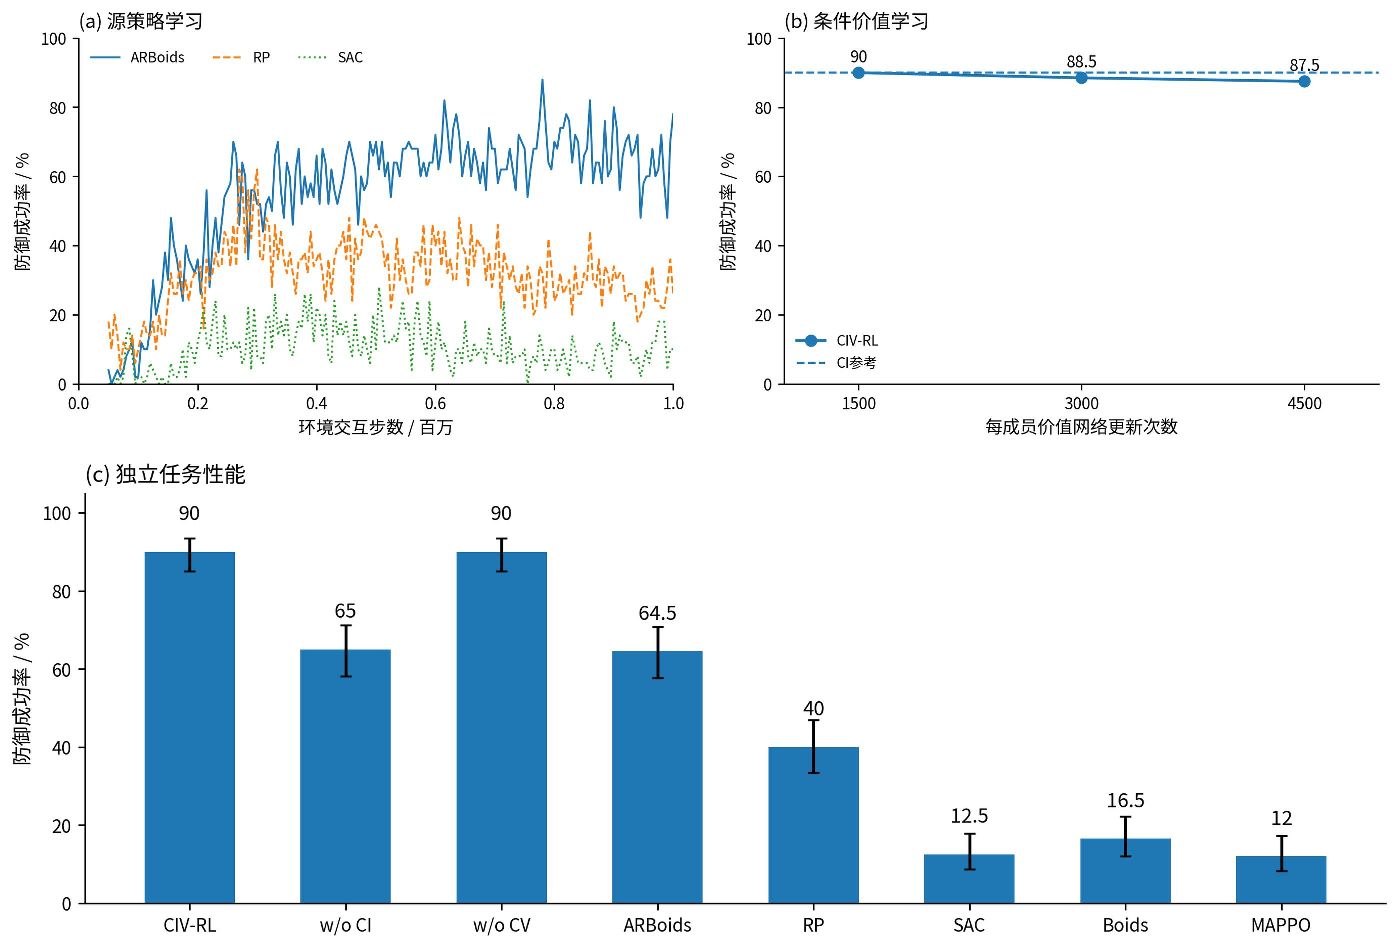
\includegraphics[width=\linewidth]{figures/fig5_performance.pdf}
\caption*{图5　学习过程与统一任务性能。（a）训练种子42对应的源策略评价记录。（b）CV实际训练检查点的闭环成功率，CI为冻结参考水平线。（c）八种冻结方法在200个配对任务上的成功率及Wilson
95\%区间。不同学习阶段分别使用环境交互步数和价值网络更新次数。}
\end{figure}

CIV-RL完成180次防御，成功率为90.0\%，95\%区间为85.06\%至93.43\%。相对于ARBoids，完整方法增加51次成功，提升25.5个百分点，艇间碰撞由70次减少至5次；相对于RP，成功率提高50.0个百分点，碰撞由115次减少至5次。完整方法的180次成功均由捕获完成，其余20次任务由5次碰撞和15次径向失守终止。上述结果将任务完成水平与失败构成同时呈现，反映了联合融合在密集六艇控制中的主要作用。

\Needspace{10\baselineskip}
\begin{center}\small\bfseries 表3　200个统一任务中的算法性能\end{center}

\begingroup
\small
\setlength{\tabcolsep}{3.2pt}
\begin{longtable}{@{}>{\raggedright\arraybackslash}p{(\linewidth - 12\tabcolsep) * \real{0.16}}
>{\raggedright\arraybackslash}p{(\linewidth - 12\tabcolsep) * \real{0.12}}
>{\raggedright\arraybackslash}p{(\linewidth - 12\tabcolsep) * \real{0.12}}
>{\raggedright\arraybackslash}p{(\linewidth - 12\tabcolsep) * \real{0.12}}
>{\raggedright\arraybackslash}p{(\linewidth - 12\tabcolsep) * \real{0.16}}
>{\raggedright\arraybackslash}p{(\linewidth - 12\tabcolsep) * \real{0.16}}
>{\raggedright\arraybackslash}p{(\linewidth - 12\tabcolsep) * \real{0.16}}@{}}
\toprule\noalign{}
\begin{minipage}[b]{\linewidth}\raggedright
方法
\end{minipage} & \begin{minipage}[b]{\linewidth}\raggedright
成功率/\%
\end{minipage} & \begin{minipage}[b]{\linewidth}\raggedright
捕获率/\%
\end{minipage} & \begin{minipage}[b]{\linewidth}\raggedright
碰撞率/\%
\end{minipage} & \begin{minipage}[b]{\linewidth}\raggedright
物理突破率/\%
\end{minipage} & \begin{minipage}[b]{\linewidth}\raggedright
径向失守率/\%
\end{minipage} & \begin{minipage}[b]{\linewidth}\raggedright
捕获时间/s
\end{minipage} \\
\midrule\noalign{}
\endhead
\bottomrule\noalign{}
\endlastfoot
CIV-RL & 90.0 & 90.0 & 2.5 & 0.0 & 7.5 & 24.02 \\
w/o CI & 65.0 & 65.0 & 34.0 & 0.0 & 1.0 & 18.78 \\
w/o CV & 90.0 & 90.0 & 2.5 & 0.0 & 7.5 & 24.84 \\
ARBoids & 64.5 & 64.5 & 35.0 & 0.0 & 0.5 & 18.86 \\
RP & 40.0 & 40.0 & 57.5 & 0.0 & 2.5 & 14.57 \\
SAC & 12.5 & 12.5 & 37.5 & 16.5 & 33.5 & 16.80 \\
Boids & 16.5 & 16.5 & 83.5 & 0.0 & 0.0 & 9.13 \\
MAPPO & 12.0 & 7.5 & 36.5 & 42.0 & 9.5 & 14.81 \\
\end{longtable}
\endgroup

w/o CI的成功率为65.0\%，完整方法增加50次成功。w/o
CV与完整方法均为90.0\%，碰撞次数均为5次。两项系统比较中，候选运动的联合配置带来主要成功率差异，条件价值选择保持相同任务完成水平。CV在1
500、3 000和4
500次更新时的冻结评价成功率分别为90.0\%、88.5\%和87.5\%，最终模型采用开发阶段确定的1
500次更新检查点。该过程反映固定联合配置结构下价值参数变化所对应的控制表现，独立完整训练的运行间统计单列于补充表S2。

\subsubsection*{4.3.2
候选交互的联合选择作用}

联合选择和独立选择共享源策略、候选控制、局部代价及预测艇对交互势。独立方法依据队友候选的局部偏好构造分布

\[
\varrho_j(\ell\mid x)
=\frac{\exp[-\phi_j(\ell;x)]}
{\sum_{q=1}^{K_j}\exp[-\phi_j(q;x)]},
\tag{39}
\]

并由各艇分别选择期望代价最小的候选

\[
k_i^{\mathrm{ind}}\in\arg\min_k
\left[\phi_i(k;x)+\lambda\sum_{j\ne i}\sum_{\ell=1}^{K_j}
\varrho_j(\ell\mid x)\psi_{ij}(k,\ell;x)\right].
\tag{40}
\]

独立选择将队友的多种候选平均纳入局部评价，联合选择则计算各艇实际共同执行的整组组合。在200个正式任务中，独立选择完成163次防御，CI完成180次，成功率由81.5\%提高至90.0\%。逐任务配对中，26个任务由失败转为成功，9个任务由成功转为失败，净增17次成功，增益为8.5个百分点，配对95\%区间为3.0至14.5个百分点。艇间碰撞由10次减少至5次。

该比较在相同候选与预测信息下改变配置的求解方式，将性能差异落实到候选之间的组合依赖。当局部偏好同时指向近距交会时，式（16）协调相关艇的融合系数，使选中的候选作为完整配置共同执行。净成功增量与碰撞减少分别反映任务结局和队内交会的变化，联合配置同时影响后续拦截位置及径向防守关系。表4汇总两项机制的直接配对结果。

\Needspace{10\baselineskip}
\begin{center}\small\bfseries 表4　候选交互与条件价值的直接比较\end{center}

\begingroup
\small
\setlength{\tabcolsep}{3.2pt}
\begin{longtable}{@{}>{\raggedright\arraybackslash}p{(\linewidth - 10\tabcolsep) * \real{0.31}}
>{\raggedright\arraybackslash}p{(\linewidth - 10\tabcolsep) * \real{0.12}}
>{\raggedright\arraybackslash}p{(\linewidth - 10\tabcolsep) * \real{0.135}}
>{\raggedright\arraybackslash}p{(\linewidth - 10\tabcolsep) * \real{0.135}}
>{\raggedright\arraybackslash}p{(\linewidth - 10\tabcolsep) * \real{0.15}}
>{\raggedright\arraybackslash}p{(\linewidth - 10\tabcolsep) * \real{0.15}}@{}}
\toprule\noalign{}
\begin{minipage}[b]{\linewidth}\raggedright
配对比较
\end{minipage} & \begin{minipage}[b]{\linewidth}\raggedright
成功数
\end{minipage} & \begin{minipage}[b]{\linewidth}\raggedright
失败转成功
\end{minipage} & \begin{minipage}[b]{\linewidth}\raggedright
成功转失败
\end{minipage} & \begin{minipage}[b]{\linewidth}\raggedright
成功率差/百分点
\end{minipage} & \begin{minipage}[b]{\linewidth}\raggedright
配对95\%区间
\end{minipage} \\
\midrule\noalign{}
\endhead
\bottomrule\noalign{}
\endlastfoot
CI相对独立选择 & 180/163 & 26 & 9 & 8.5 & {[}3.0, 14.5{]} \\
CIV-RL相对仅CI & 180/180 & 4 & 4 & 0.0 & {[}−3.0, 2.5{]} \\
CV相对普通价值 & 180/179 & 4 & 3 & 0.5 & {[}−2.0, 3.0{]} \\
\end{longtable}
\endgroup

\subsubsection*{4.3.3
条件价值与完整融合选择}

条件价值模型与普通终局价值模型使用相同CI参考、配对初始状态、联合候选和关系网络。普通模型以完整方案成功标签监督输出，条件模型采用式（29）至式（31）拟合参考事件下的候选后果与净收益。两类模型使用相同候选接受规则和开发验证协议，所选方案通过相同的反馈控制过程执行。

完整CIV-RL在200个任务中接受38次候选，其中4个任务由参考失败转为成功，4个任务由参考成功转为失败，最终与仅CI均完成180次防御。普通价值模型完成179次防御，条件价值模型相对其形成4次失败转成功和3次成功转失败。对于完整方法与仅CI共同捕获的176个任务，平均配对捕获时间缩短0.83
s；两者各自捕获回合的平均时间分别为24.02 s和24.84
s。条件价值选择在保持该组任务成功率的同时改变了部分拦截过程，共同捕获任务给出了时间变化的对应观察。

候选辨识进一步在未参与拟合的配对初始状态上评价。设\(\mathcal P_{\ne}\)为经验价值存在差异的候选对集合，排序一致率和净收益误差定义为

\[
\begin{aligned}
A_{\mathrm{ord}}
&=\frac1{|\mathcal P_{\ne}|}
\sum_{(x,z,z')\in\mathcal P_{\ne}}
\mathbb I\!\left[\Delta_\theta(x;z,z')\widehat\Delta(x;z,z')>0\right],\\
E_\Delta&=\mathbb E\!\left[
\bigl(\Delta_\theta(x;z,z')-\widehat\Delta(x;z,z')\bigr)^2\right].
\end{aligned}
\tag{41}
\]

CV与普通价值模型的排序一致率分别为［　］和［　］，收益误差分别为［　］和［　］。该评价使用候选方案的配对终局结果，表4使用完整任务中的实际选择结果，二者分别对应价值辨识与价值参与后的控制表现。

\subsubsection*{4.3.4
交互权重与接受阈值}

关键参数在100个共同开发任务中比较。CI采用\(\lambda\in\{0,16,32,64\}\)时，成功率分别为66.0\%、91.0\%、91.0\%和89.0\%，碰撞次数分别为34、2、3和4。加入艇对项后，联合配置同时取得较高任务完成水平和较低碰撞次数。在16至64的取值范围内，成功率保持89.0\%至91.0\%，体现名义权重附近可用的交互调节区间。

固定价值网络与候选空间时，\(\varepsilon\in\{0,0.025,0.075,0.15\}\)对应的成功率为95.0\%、95.0\%、95.0\%和92.0\%，接受次数依次为71、49、16和2。阈值从0增加至0.075时，候选执行次数减少55次，最终成功率保持95.0\%；配对变化由6次失败转成功和2次成功转失败，转为4次失败转成功及零次成功转失败。接受门槛由此调节候选执行频率及成败转化组合。补充表S1分别注明两组比较的参考策略，正式主评价使用冻结的\(\lambda=32\)和\(\varepsilon=0.075\)。

\subsection*{4.4
攻击者机动性}

机动性试验固定六艘防御艇，使用同一源策略、CI参数和条件价值模型，攻击机动系数取1.0、1.5、2.0、2.5、3.0和3.5，每个等级评价24个任务。同一等级内，各方法使用配对初始几何与随机条件。图6(a)给出完整方法、仅CI、ARBoids与RP的防御成功率。

CIV-RL在六个机动等级分别完成22、22、19、23、23和15次防御，成功率依次为91.67\%、91.67\%、79.17\%、95.83\%、95.83\%和62.50\%。在\(L_{\mathrm{agi}}=2.5\)和3.0时，完整方法均完成23次防御且未发生艇间碰撞，ARBoids分别完成18次和15次，RP分别完成13次和9次。候选交互在该机动范围内维持了较高捕获水平与运动分离。

不同等级下的结果呈现非单调变化。\(L_{\mathrm{agi}}=3.5\)时，CIV-RL与ARBoids均完成15次防御，碰撞次数分别为3次和9次，表明在相同成功数下，两种方法形成了不同的队内交会结果。图6(a)按各等级的共同任务分别统计，成功率和失败构成共同描述攻击者机动变化下的控制表现。

\subsection*{4.5
未见艇队规模}

规模评价使用六艇训练完成的冻结源策略和条件价值模型，测试3、4、5、7和8艘防御艇，每个未见规模使用24个配对任务。六艇参考点由机动系数2.0和2.5下的48个任务组成。CI依据当前艇队构造候选交互，CV通过共享节点映射及艇队聚合评价相应完整方案，各规模沿用相同参数和接受规则。图6(b)给出完整控制器的跨规模表现。

\begin{figure}[!htbp]
\centering
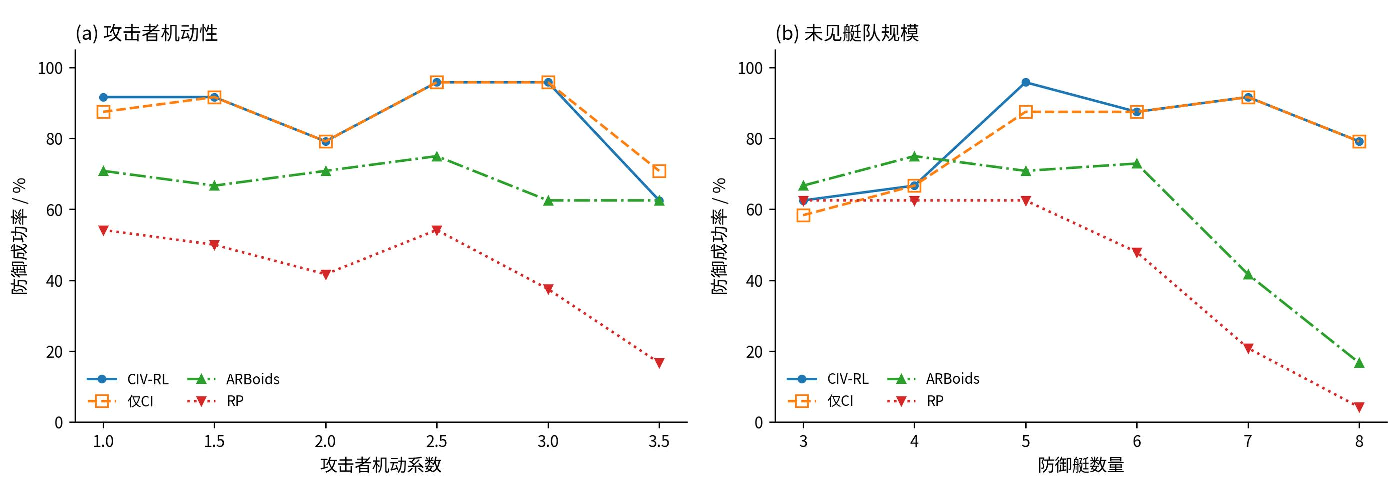
\includegraphics[width=\linewidth]{figures/fig6_scope.pdf}
\caption*{图6　冻结策略的机动性与规模评价。（a）六艇条件下每个机动等级使用24个配对任务。（b）每个未见艇数使用24个任务，六艇参考点使用48个任务。完整方法与仅CI曲线重合处采用不同线型和空心标记。}
\end{figure}

在5、7和8艘艇条件下，CIV-RL分别完成23/24、22/24和19/24次防御，ARBoids分别完成17/24、10/24和4/24次。对应碰撞次数，完整方法为0、0和4次，ARBoids为5、14和20次。艇数增大时，同时发生的候选运动关系增多，联合配置在这些条件下通过调整候选组合保持了较好的艇间分离，较大艇队中的成功率差异也更突出。

在3艇和4艇条件下，完整方法分别完成15/24和16/24次防御，ARBoids分别完成16/24和18/24次。小艇队中的目标覆盖与个体到达能力对捕获过程具有较大影响。相对于仅CI，完整方法在3艇和5艇条件下分别增加1次和2次成功，其余规模成功数相同。共享关系表示使价值模型能够读取变长艇队输入，冻结任务结果则评价该表示与联合选择在不同规模中的实际使用效果。

CI对当前所有不同防御艇对计算交互项，图中测试规模对应的无向交互边数为\(n(n-1)/2\)。从3艇增加至8艇时，边数由3增至28，交互权重保持不变；配置搜索和候选价值评价的计算量随有效艇数变化。候选预测和联合求解沿用相同计算配置，规模变化的计算量由有效艇数和保留候选数共同确定。

\subsection*{4.6
学习型攻击者与条件价值更新}

对手试验先冻结CIV-RL，使已训练的SAC攻击者继续与该防御策略交互，随后固定更新后的攻击者，并使用新的配对闭环结果更新条件价值模型。攻击阶段新增32
883步环境交互，在新增0、8 000、16 000和32
883步时使用相同64个任务评价。完整方法分别完成55、59、55和59次防御，碰撞次数分别为1、1、0和0，防御成功率处于85.94\%至92.19\%。图7(a)以实际新增交互量表示攻击者继续学习阶段。

防御更新阶段从当前攻击策略下的192个任务中取得190个可行动初始状态，每个状态使用两组共同随机序列，共生成4
180条闭环分支。CI保持固定，条件价值模型根据当前对手的终局后果继续拟合。随后将原人工势场任务的参考与候选观测共同纳入价值训练，评价对当前对手的适应和原任务保持。

\begin{figure}[!htbp]
\centering
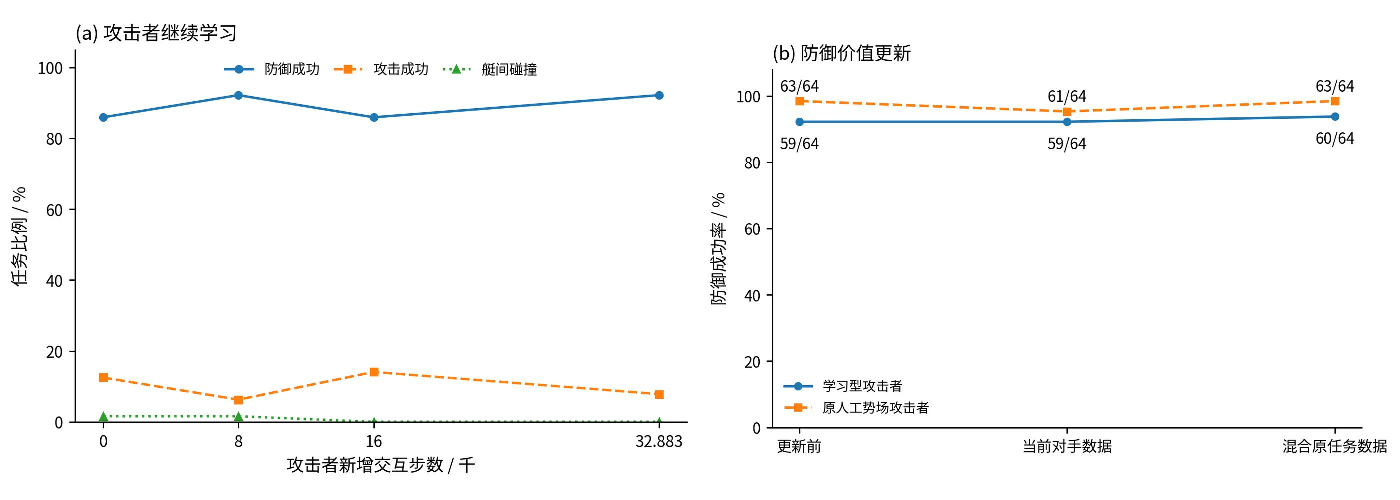
\includegraphics[width=\linewidth]{figures/fig7_adaptation.pdf}
\caption*{图7　学习型攻击者与防御价值更新。（a）攻击者继续学习时的64任务评价，横轴为新增环境交互步数。（b）防御更新前、当前对手数据更新后与混合原任务数据后，在两类对手下的成功率，标注对应成功数。}
\end{figure}

在最终学习型攻击者下，防御更新前、当前对手数据更新后和加入原任务数据后，CIV-RL分别完成59/64、59/64和60/64次防御；原人工势场攻击者下对应为63/64、61/64和63/64次。混合两类任务观测后，方法分别取得93.75\%和98.44\%的成功率，两组评价均未出现艇间碰撞。当前对手数据更新保留了学习型攻击任务的成功数，原任务数据的加入恢复了原人工势场条件下的成功数，并增加一次学习型攻击者下的防御成功。该过程体现了在固定联合融合结构中利用新闭环后果更新候选任务价值的方式。

\FloatBarrier\section*{5 结论}

本文针对多无人艇目标防御中的融合控制耦合，提出候选交互与条件价值驱动的协同控制方法CIV-RL。以左右推进器融合系数为整队决策变量，通过反馈运动预测构建艇对候选交互，结合源策略融合偏好联合确定控制配置。配对闭环条件价值学习分别估计参考失败与成功事件下的候选结果，将成败转化的净收益用于同一候选空间中的最终方案选择。

六艇独立任务中，所提方法取得90.0\%的防御成功率，较ARBoids提高25.5个百分点，碰撞率由35.0\%降至2.5\%。共享候选与预测信息的比较给出8.5个百分点的联合选择增益，支持在整队配置上处理局部融合控制的组合依赖。条件价值参与后保持相同防御成功率，并在共同捕获任务上缩短平均捕获时间。12组VRX配对场景均完成捕获，机动性、跨艇数和对手继续学习试验进一步给出完整控制器在不同任务条件下的执行表现。

\FloatBarrier\section*{参考文献}\begingroup\small\setlength{\parindent}{0pt}\setlength{\parskip}{4pt}

{[}1{]} Qiao Y, Yin J, Wang W, et al.~Survey of deep learning for
autonomous surface vehicles in marine environments. IEEE Transactions on
Intelligent Transportation Systems, 2023, 24(4), 3678-3701. DOI
10.1109/TITS.2023.3235911.

{[}2{]} Fu H, Liu H H T. Guarding a territory against an intelligent
intruder: Strategy design and experimental verification. IEEE/ASME
Transactions on Mechatronics, 2020, 25(4), 1765-1772. DOI
10.1109/TMECH.2020.2996901.

{[}3{]} Chen Y, Wu Y, Yang H, et al.~A distributed pipeline for
collaborative pursuit in the target guarding problem. IEEE Robotics and
Automation Letters, 2024, 9(3), 2064-2071. DOI 10.1109/LRA.2024.3349977.

{[}4{]} Yan R, Duan X, Zou R, et al.~Multiplayer homicidal chauffeur
reach-avoid games: A pursuit enclosure function approach. Automatica,
2024, 167, 111770. DOI 10.1016/j.automatica.2024.111770.

{[}5{]} Fang X, Wang C, Xie L, Chen J. Cooperative pursuit with
multi-pursuer and one faster free-moving evader. IEEE Transactions on
Cybernetics, 2022, 52(3), 1405-1414. DOI 10.1109/TCYB.2019.2958548.

{[}6{]} Guo X, Cui R, Yan W. Pursuit-evasion games of marine surface
vessels using neural network-based control. IEEE Transactions on
Systems, Man, and Cybernetics: Systems, 2025, 55(1), 18-27. DOI
10.1109/TSMC.2023.3347044.

{[}7{]} Reynolds C W. Flocks, herds and schools: A distributed
behavioral model. Computer Graphics, 1987, 21(4), 25-34. DOI
10.1145/37402.37406.

{[}8{]} de Souza C, Newbury R, Cosgun A, et al.~Decentralized
multi-agent pursuit using deep reinforcement learning. IEEE Robotics and
Automation Letters, 2021, 6(3), 4552-4559. DOI 10.1109/LRA.2021.3068952.

{[}9{]} 夏家伟，朱旭芳，张建强，罗亚松，刘忠.
基于多智能体强化学习的无人艇协同围捕方法.
控制与决策，2023，38(5)，1438-1447. DOI 10.13195/j.kzyjc.2022.0564.

{[}10{]} Xue S, Zhao N, Wang L, et al.~Multi-agent self-attention
reinforcement learning for multi-USV hunting target. Neural Networks,
2025, 189, 107574. DOI 10.1016/j.neunet.2025.107574.

{[}11{]} Yu J, et al.~A cooperative hunting method for multi-USVs based
on trajectory prediction by OR-LSTM. IEEE Transactions on Vehicular
Technology, 2024, 73(12), 18087-18101. DOI 10.1109/TVT.2024.3432739.

{[}12{]} Hüttenrauch M, Šošić A, Neumann G. Deep reinforcement learning
for swarm systems. Journal of Machine Learning Research, 2019, 20(54),
1-31.

{[}13{]} Rashid T, Samvelyan M, de Witt C S, et al.~Monotonic value
function factorisation for deep multi-agent reinforcement learning.
Journal of Machine Learning Research, 2020, 21(178), 1-51.

{[}14{]} Yu C, Velu A, Vinitsky E, et al.~The surprising effectiveness
of PPO in cooperative multi-agent games. Advances in Neural Information
Processing Systems, 2022, 35, 24611-24624.

{[}15{]} Boehmer W, Kurin V, Whiteson S. Deep coordination graphs.
Proceedings of the 37th International Conference on Machine Learning,
2020, 119, 980-991.

{[}16{]} Ma Z, Luo Y, Pan J. Learning selective communication for
multi-agent path finding. IEEE Robotics and Automation Letters, 2022,
7(2), 1455-1462. DOI 10.1109/LRA.2021.3139145.

{[}17{]} Li Q, Lin W, Liu Z, Prorok A. Message-aware graph attention
networks for large-scale multi-robot path planning. IEEE Robotics and
Automation Letters, 2021, 6(3), 5533-5540. DOI 10.1109/LRA.2021.3077863.

{[}18{]} Johannink T, Bahl S, Nair A, et al.~Residual reinforcement
learning for robot control. Proceedings of the IEEE International
Conference on Robotics and Automation, 2019, 6023-6029. DOI
10.1109/ICRA.2019.8794127.

{[}19{]} Rana K, et al.~Bayesian controller fusion: Leveraging control
priors in deep reinforcement learning for robotics. The International
Journal of Robotics Research, 2023, 42(3), 123-146. DOI
10.1177/02783649231167210.

{[}20{]} Jeon S H, Lee H J, Hong S, Kim S. Residual MPC: Blending
reinforcement learning with GPU-parallelized model predictive control.
arXiv, 2025, 2510.12717.

{[}21{]} Tao J, Shen T, Zhao D, Zhang F. ARBoids: Adaptive residual
reinforcement learning with Boids model for cooperative multi-USV target
defense. IEEE Robotics and Automation Letters, 2026, 11(3), 3637-3644.
DOI 10.1109/LRA.2026.3662620.

{[}22{]} Foerster J, Farquhar G, Afouras T, et al.~Counterfactual
multi-agent policy gradients. Proceedings of the AAAI Conference on
Artificial Intelligence, 2018, 32(1), 2974-2982. DOI
10.1609/aaai.v32i1.11794.

{[}23{]} Bhattacharya S, Kailas S, Badyal S, Gil S, Bertsekas D.
Multiagent reinforcement learning: Rollout and policy iteration for
POMDP with application to multirobot problems. IEEE Transactions on
Robotics, 2024, 40, 2003-2023. DOI 10.1109/TRO.2023.3347128.

{[}24{]} Feinberg V, Wan A, Stoica I, Jordan M I, Gonzalez J E, Levine
S. Model-based value estimation for efficient model-free reinforcement
learning. arXiv, 2018, 1803.00101.

{[}25{]} Fossen T I. Handbook of Marine Craft Hydrodynamics and Motion
Control. Chichester, Wiley, 2011.

{[}26{]} Bingham B, Aguero C, McCarrin M, et al.~Toward maritime robotic
simulation in Gazebo. Proceedings of the MTS/IEEE OCEANS Conference,
2019, 1-10. DOI 10.23919/OCEANS40490.2019.8962725.

{[}27{]} Haarnoja T, Zhou A, Abbeel P, Levine S. Soft actor-critic:
Off-policy maximum entropy deep reinforcement learning with a stochastic
actor. Proceedings of the 35th International Conference on Machine
Learning, 2018, 80, 1861-1870.

{[}28{]} Bengio Y, Louradour J, Collobert R, Weston J. Curriculum
learning. Proceedings of the 26th Annual International Conference on
Machine Learning, 2009, 41-48. DOI 10.1145/1553374.1553380.

\endgroup\clearpage\section*{补充材料}

\subsection*{S1
关键参数与配对任务结果}

交互权重分析固定源策略、候选集合和预测时域，在同一组100个开发任务中改变艇对代价权重，配对参考为\(\lambda_0=32\)的CI。接受阈值分析固定CI与CV模型，配对参考为同一名义CI。表S1中的净增量分别按照上述参考计算，候选接受次数仅用于条件价值选择。

\Needspace{10\baselineskip}
\begin{center}\small\bfseries 表S1　交互权重与接受阈值敏感性\end{center}

\begingroup
\small
\setlength{\tabcolsep}{3.2pt}
\begin{longtable}{@{}>{\raggedright\arraybackslash}p{(\linewidth - 14\tabcolsep) * \real{0.18}}
>{\raggedright\arraybackslash}p{(\linewidth - 14\tabcolsep) * \real{0.1}}
>{\raggedright\arraybackslash}p{(\linewidth - 14\tabcolsep) * \real{0.12}}
>{\raggedright\arraybackslash}p{(\linewidth - 14\tabcolsep) * \real{0.11}}
>{\raggedright\arraybackslash}p{(\linewidth - 14\tabcolsep) * \real{0.1}}
>{\raggedright\arraybackslash}p{(\linewidth - 14\tabcolsep) * \real{0.14}}
>{\raggedright\arraybackslash}p{(\linewidth - 14\tabcolsep) * \real{0.14}}
>{\raggedright\arraybackslash}p{(\linewidth - 14\tabcolsep) * \real{0.11}}@{}}
\toprule\noalign{}
\begin{minipage}[b]{\linewidth}\raggedright
参数
\end{minipage} & \begin{minipage}[b]{\linewidth}\raggedright
取值
\end{minipage} & \begin{minipage}[b]{\linewidth}\raggedright
成功率/\%
\end{minipage} & \begin{minipage}[b]{\linewidth}\raggedright
碰撞数
\end{minipage} & \begin{minipage}[b]{\linewidth}\raggedright
接受数
\end{minipage} & \begin{minipage}[b]{\linewidth}\raggedright
失败转成功
\end{minipage} & \begin{minipage}[b]{\linewidth}\raggedright
成功转失败
\end{minipage} & \begin{minipage}[b]{\linewidth}\raggedright
净增/百分点
\end{minipage} \\
\midrule\noalign{}
\endhead
\bottomrule\noalign{}
\endlastfoot
\(\lambda/\lambda_0\) & 0.0 & 66.0 & 34 & 0 & 4 & 29 & −25.0 \\
\(\lambda/\lambda_0\) & 0.5 & 91.0 & 2 & 0 & 6 & 6 & 0.0 \\
\(\lambda/\lambda_0\) & 1.0 & 91.0 & 3 & 0 & 0 & 0 & 0.0 \\
\(\lambda/\lambda_0\) & 2.0 & 89.0 & 4 & 0 & 4 & 6 & −2.0 \\
\(\varepsilon\) & 0.000 & 95.0 & 3 & 71 & 6 & 2 & 4.0 \\
\(\varepsilon\) & 0.025 & 95.0 & 3 & 49 & 6 & 2 & 4.0 \\
\(\varepsilon\) & 0.075 & 95.0 & 3 & 16 & 4 & 0 & 4.0 \\
\(\varepsilon\) & 0.150 & 92.0 & 3 & 2 & 1 & 0 & 1.0 \\
\end{longtable}
\endgroup

\subsection*{S2
独立完整训练统计}

完整训练运行以源策略、相应CI配置及其配对条件价值学习为统计单元。各运行采用相同训练设置和正式任务分布，源策略及价值模型分别使用独立随机初始化。表S2记录运行数、任务成功率均值、运行间标准差及相对既定参考的平均配对差。

\Needspace{10\baselineskip}
\begin{center}\small\bfseries 表S2　独立完整训练结果\end{center}

\begingroup
\small
\setlength{\tabcolsep}{3.2pt}
\begin{longtable}{@{}>{\raggedright\arraybackslash}p{(\linewidth - 14\tabcolsep) * \real{0.26}}
>{\raggedright\arraybackslash}p{(\linewidth - 14\tabcolsep) * \real{0.10571}}
>{\raggedright\arraybackslash}p{(\linewidth - 14\tabcolsep) * \real{0.10571}}
>{\raggedright\arraybackslash}p{(\linewidth - 14\tabcolsep) * \real{0.10571}}
>{\raggedright\arraybackslash}p{(\linewidth - 14\tabcolsep) * \real{0.10571}}
>{\raggedright\arraybackslash}p{(\linewidth - 14\tabcolsep) * \real{0.10571}}
>{\raggedright\arraybackslash}p{(\linewidth - 14\tabcolsep) * \real{0.10571}}
>{\raggedright\arraybackslash}p{(\linewidth - 14\tabcolsep) * \real{0.10571}}@{}}
\toprule\noalign{}
\begin{minipage}[b]{\linewidth}\raggedright
统计量
\end{minipage} & \begin{minipage}[b]{\linewidth}\raggedright
CIV-RL
\end{minipage} & \begin{minipage}[b]{\linewidth}\raggedright
w/o CI
\end{minipage} & \begin{minipage}[b]{\linewidth}\raggedright
w/o CV
\end{minipage} & \begin{minipage}[b]{\linewidth}\raggedright
ARBoids
\end{minipage} & \begin{minipage}[b]{\linewidth}\raggedright
RP
\end{minipage} & \begin{minipage}[b]{\linewidth}\raggedright
SAC
\end{minipage} & \begin{minipage}[b]{\linewidth}\raggedright
MAPPO
\end{minipage} \\
\midrule\noalign{}
\endhead
\bottomrule\noalign{}
\endlastfoot
完整训练运行数 & ［　］ & ［　］ & ［　］ & ［　］ & ［　］ & ［　］ &
［　］ \\
防御成功率均值 & ［　］ & ［　］ & ［　］ & ［　］ & ［　］ & ［　］ &
［　］ \\
运行间标准差 & ［　］ & ［　］ & ［　］ & ［　］ & ［　］ & ［　］ &
［　］ \\
相对参考的平均配对差 & ［　］ & ［　］ & ［　］ & ［　］ & ［　］ &
［　］ & ［　］ \\
\end{longtable}
\endgroup

\end{document}
